\documentclass[10pt]{ctexart}
\usepackage{listings}
\usepackage{amsmath} 
\usepackage{amssymb} 
\usepackage{xcolor}
\usepackage{xeCJK}
\usepackage{fontspec}
\usepackage{titlesec}
\usepackage{titletoc}
\usepackage{setspace}
\usepackage{graphicx}
\usepackage{geometry}
\usepackage[T1]{fontenc}  
\usepackage{textcomp}  
\usepackage{lmodern}
\usepackage[colorlinks,
            linkcolor=black,
            anchorcolor=black,
            citecolor=black]{hyperref}
\geometry{a4paper,scale=0.8}
\renewcommand\contentsname{Contents}
\setmonofont[Mapping={}]{Monaco}    %英文引号之类的正常显示,相当于设置英文字体
%\setsansfont{Consolas} %设置英文字体 Monaco, Consolas,  Fantasque Sans Mono
%\setmainfont{Monaco} %设置英文字体
% 定义可能使用到的颜色
%\setmainfont[BoldFont=SimHei]{SimSun}
\definecolor{CPPLight}  {HTML} {686868}
\definecolor{CPPSteel}  {HTML} {888888}
\definecolor{CPPDark}   {HTML} {262626}
\definecolor{CPPBlue}   {HTML} {4172A3}
\definecolor{CPPGreen}  {HTML} {487818}
\definecolor{CPPBrown}  {HTML} {A07040}
\definecolor{CPPRed}    {HTML} {AD4D3A}
\definecolor{CPPViolet} {HTML} {7040A0}
\definecolor{CPPGray}  {HTML} {B8B8B8}
\lstset{
    columns=fixed,       
    numbers=left,                                        % 在左侧显示行号
    frame=none,                                          % 不显示背景边框
    backgroundcolor=\color[RGB]{245,245,244},            % 设定背景颜色
    keywordstyle=\color[RGB]{40,40,255},                 % 设定关键字颜色
    numberstyle=\small\color{darkgray},                  % 设定行号格式
    commentstyle=\it\color[RGB]{0,96,96},                % 设置代码注释的格式
    stringstyle=\rmfamily\slshape\color[RGB]{128,0,0},   % 设置字符串格式
    showstringspaces=false,                              % 不显示字符串中的空格
    language=c++,                                        % 设置语言
    morekeywords={alignas,continute,friend,register,true,alignof,decltype,goto,
    reinterpret_cast,try,asm,defult,if,return,typedef,auto,delete,inline,short,
    typeid,bool,do,int,signed,typename,break,double,long,sizeof,union,case,
    dynamic_cast,mutable,static,unsigned,catch,else,namespace,static_assert,using,
    char,enum,new,static_cast,virtual,char16_t,char32_t,explict,noexcept,struct,
    void,export,nullptr,switch,volatile,class,extern,operator,template,wchar_t,
    const,false,private,this,while,constexpr,float,protected,thread_local,
    const_cast,for,public,throw,std},
    emph={map,set,multimap,multiset,unordered_map,unordered_set,
    unordered_multiset,unordered_multimap,vector,string,list,deque,
    array,stack,forwared_list,iostream,memory,shared_ptr,unique_ptr,
    random,bitset,ostream,istream,cout,cin,endl,move,default_random_engine,
    uniform_int_distribution,iterator,algorithm,functional,bing,numeric,},
    emphstyle=\color{CPPViolet},
    basicstyle=\linespread{1}\small\fontspec{Courier New Bold}\ttfamily,
    breaklines=true,
    %xleftmargin=1em,xrightmargin=1em, aboveskip=1em,
    % in the listings package configuration, try:  
    literate={"}{\textquotedbl}1,  
    tabsize=4, keepspaces=true
}
%\setmainfont{Courier New Bold}
%\begin{lstlisting}

%\end{lstlisting}
\CTEXoptions[today=old]
\title{TEMPLATE}
\author{}
\date{Last build at \today}

\begin{document}{
\begin{titlepage}
    \centering
    \vspace{2cm}
    {\scshape\Large South China University of Technology \par}
    \vspace{1cm}
    {\scshape\Large SCUT\_gugugu\par}
    \vspace{1.5cm}
    {\Huge\bfseries TEMPLATE\par}
    \vspace{4.5cm}
    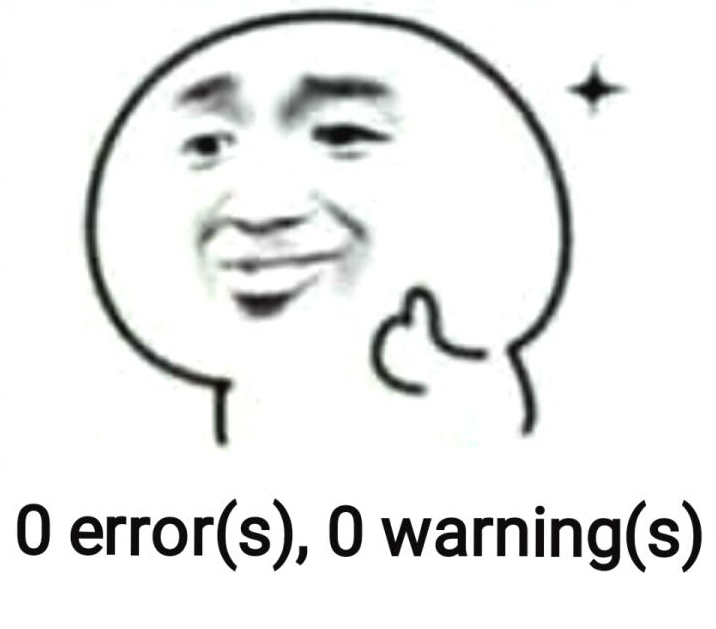
\includegraphics[width=0.5\textwidth]{./LOGO}\par\vspace{1cm}
    %\vspace{5cm}
    %{\Large\itshape Nickwzk\par}

    \vfill

% Bottom of the page
    {\large Last build at \today\par}

%\setcounter{page}{0}
\thispagestyle{empty}
%\newpage
\end{titlepage}
\tableofcontents
\newpage
\section{Graph Theory}
\subsection{Shortest Path}
\subsubsection{Dijkstra}
\begin{lstlisting}
typedef pair<int, int> P;
struct Edge {
    int to, nxt;
    LL w;
}e[MAXM];
int head[MAXN], ecnt;
LL d[MAXN];
priority_queue<P, vector<P>, greater<P> > q;
inline void addEdge(int x, int y, LL w) {
    e[++ecnt] = (Edge) {y, head[x], w}; head[x] = ecnt;
}
void dijkstra(int st) {
    memset(d, 0x3f, sizeof(d));
    d[st] = 0;
    q.push(make_pair(0, st));
    while(!q.empty()) {
        P x = q.top(); q.pop();
        int u = x.second;
        for(int i = head[u], v; i; i = e[i].nxt) {
            v = e[i].to;
            if(d[v] > d[u] + e[i].w) {
                d[v] = d[u] + e[i].w;
                q.push(make_pair(d[v], v));
            }
        }
    }
}
\end{lstlisting}
\subsubsection{SPFA}
\begin{lstlisting}
struct Edge {
    int to, nxt;
    LL w;
}e[MAXE];
int head[MAXN], ecnt;
LL d[MAXN];
bool exist[MAXN];
queue<int> q;
inline void addEdge(int x, int y, LL w) {
   e[++ecnt] = (Edge) {y, head[x], w}; head[x] = ecnt;
}
void SPFA(int st) {
    memset(d,0x3f,sizeof(d));
    d[st] = 0;
    q.push(st);
    exist[st] = 1;
    while(!q.empty()) {
        int u = q.front(); q.pop();
        exist[u] = 0;
        for(int i = head[u], v; i; i = e[i].nxt) {
            v = e[i].to;
            if(d[v] > d[u] + e[i].w) {
                d[v] = d[u] + e[i].w;
                //pre[v] = u;
                if(!exist[v]) {
                    q.push(v);
                    exist[v] = 1;
                }
            }
        }
    }
}
\end{lstlisting}
\subsection{Network Flow}
\subsubsection{ISAP}
\begin{lstlisting}
namespace NWF {
    struct Edge{
        int to, nxt;LL f;
    }e[MAXM << 1];
    int S, T, tot;
    int ecnt, head[MAXN], cur[MAXN], pre[MAXN], num[MAXN], dis[MAXN];
    queue<int> q;
    void init(int _S, int _T, int _tot){
        ecnt = 1; S = _S; T = _T; tot = _tot;
        memset(num,  0, (tot + 1) * sizeof(int));
        memset(head, 0, (tot + 1) * sizeof(int));
    } 
    inline void addEdge(int u, int v, LL f) {
        e[++ecnt] = (Edge) {v, head[u], f}; head[u] = ecnt;
        e[++ecnt] = (Edge) {u, head[v], 0}; head[v] = ecnt;
    }
    void bfs() {
        memset(dis, 0, (tot + 1) * sizeof(int));
        q.push(T);
        dis[T] = 1;
        while(!q.empty()) {
            int u = q.front(), v; q.pop();
            num[dis[u]]++;
            for(int i = cur[u] = head[u]; i; i = e[i].nxt) {
                if(!dis[v = e[i].to]) {
                    dis[v] = dis[u] + 1;
                    q.push(v);
                }
            }
        }
    }
    LL augment() {
        LL flow = INF;
        for(int i = S; i != T; i = e[cur[i]].to) 
            flow = min(flow, e[cur[i]].f);
        for(int i = S; i != T; i = e[cur[i]].to) {
            e[cur[i]].f -= flow;
            e[cur[i] ^ 1].f += flow;
        }
        return flow;
    }
    LL isap() {
        bfs();
        int u = S, v;
        LL flow = 0;
        while(dis[S] <= tot) {
            if(u == T) {
                flow += augment();
                u = S;
            }
            bool fg = 0;
            for(int i = cur[u]; i; i = e[i].nxt) {
                if(e[i].f && dis[u] > dis[v = e[i].to]) {
                    pre[v] = u;
                    cur[u] = i;
                    u = v;
                    fg = 1;
                    break;
                }
            }
            if(fg) continue;
            if(!--num[dis[u]]) break;
            int maxDis = tot;
            for(int i = head[u]; i; i = e[i].nxt) {
                if(e[i].f && maxDis > dis[v = e[i].to]) {
                    maxDis = dis[v];
                    cur[u] = i;
                }
            }
            num[dis[u] = maxDis + 1]++;
            if(u != S) u = pre[u];
        }
        return flow;
    }
}
\end{lstlisting}
\subsubsection{HLPP}
\begin{lstlisting}
namespace NWF{
    struct Edge{
        int to,nxt;LL f;
    }e[MAXM << 1];
    int S, T, tot;
    int ecnt, head[MAXN], dis[MAXN], num[MAXN];
    LL sumf[MAXN];
    queue<int> q;
    list<int> dep[MAXN];
    void init(int _S,int _T,int _tot){
        ecnt = 1;S = _S;T = _T;tot = _tot;
        memset(num,  0, (tot + 1) * sizeof(int));
        memset(head, 0, (tot + 1) * sizeof(int));
        memset(sumf, 0, (tot + 1) * sizeof(LL));
    }
    void addEdge(int u,int v,LL f){
        e[++ecnt] = (Edge) {v, head[u], f};head[u] = ecnt;
        e[++ecnt] = (Edge) {u, head[v], 0};head[v] = ecnt;
    }
    void bfs(){
        memset(dis, 0, (tot + 1) * sizeof(int));
        q.push(T); dis[T] = 1;
        while(!q.empty()){
            int u=q.front(), v; q.pop();
            for(int i = head[u]; i; i = e[i].nxt)
            if(!dis[v = e[i].to]){
                dis[v] = dis[u] + 1;
                q.push(v);
            }
        }
    }
    LL hlpp(){
        bfs();
        dis[S] = tot + 1;
        for(int i = 1;i <= tot; ++i)num[dis[i]]++;
        for(int i = tot + 1; ~i; --i)dep[i].clear();
        int maxd = dis[S];LL f;
        dep[maxd].push_back(S);sumf[S] = INF;
        for(;;){
            while(maxd && dep[maxd].empty())maxd--;
            if(!maxd)break;
            int u = dep[maxd].back(), v;dep[maxd].pop_back();
            int minDis = tot + 1;
            for(int i = head[u]; i;i = e[i].nxt)
            if(e[i].f){
                if(dis[u] > dis[v = e[i].to]){
                    f = min(sumf[u], e[i].f);
                    e[i].f -= f;e[i^1].f += f;
                    if(sumf[u] != INF) sumf[u] -= f;
                    if(sumf[v] != INF) sumf[v] += f; 
                    if(v!=S && v!=T && sumf[v] == f){
                        maxd = max(maxd, dis[v]);
                        dep[dis[v]].push_back(v);
                    }
                    if(!sumf[u])break;
                }else minDis=min(minDis, dis[v] + 1);
            }
            if(sumf[u]){
                if(!--num[dis[u]]){
                    for(int i = dis[u];i <= maxd;++i){
                        while(!dep[i].empty()){
                            --num[i];
                            dis[dep[i].back()] = tot + 1;
                            dep[i].pop_back();
                        }
                    }
                    maxd = dis[u] - 1;dis[u] = tot + 1;
                }else{
                    dis[u] = minDis;
                    if(minDis > tot)continue;
                    num[minDis]++;
                    maxd = max(maxd, minDis);
                    dep[minDis].push_back(u);
                }
            }
        }
        return sumf[T];
    }
}
\end{lstlisting}
\subsubsection{Dinic}
\begin{lstlisting}
namespace NWF {
    struct Edge {
        int to, nxt;LL f;
    } e[MAXM << 1]; 
    int S, T, tot;
    int ecnt, head[MAXN], cur[MAXN], dis[MAXN];
    queue<int> q;
    void init(int _S, int _T, int _tot){
        ecnt = 1; S = _S; T = _T; tot = _tot;
        memset(head, 0, (tot + 1) * sizeof(int));
    } 
    void addEdge(int u, int v, LL f) {
        e[++ecnt] = (Edge) {v, head[u], f}; head[u] = ecnt;
        e[++ecnt] = (Edge) {u, head[v], 0}; head[v] = ecnt;
    }
    bool bfs() {
        memset(dis, 0, (tot + 1) * sizeof(int));
        q.push(S); dis[S] = 1;
        while (!q.empty()) {
            int u = q.front(), v; q.pop();
            for (int i = cur[u] = head[u]; i ; i = e[i].nxt) {
                if (e[i].f && !dis[v = e[i].to]) {
                    q.push(v);
                    dis[v] = dis[u] + 1;
                }
            }
        }
        return dis[T];
    }
    LL dfs(int u, LL maxf) {
        if (u == T) return maxf;
        LL sumf = maxf;
        for (int &i = cur[u]; i; i = e[i].nxt) {
            if (e[i].f && dis[e[i].to] > dis[u]) {
                LL tmpf = dfs(e[i].to, min(sumf, e[i].f));
                e[i].f -= tmpf; e[i ^ 1].f += tmpf;
                sumf -= tmpf;
                if (!sumf) return maxf;
            }
        }
        return maxf - sumf;
    }
    LL dinic() {
        LL ret = 0;
        while (bfs()) ret += dfs(S, INF);
        return ret;
    }
}
\end{lstlisting}
\subsubsection{MCMF}
\begin{lstlisting}
namespace NWF{
    struct Edge {
        int to, nxt;LL f, c;
    } e[MAXM << 1]; 
    int S, T, tot;
    int ecnt, head[MAXN], cur[MAXN];LL dis[MAXN];
    bool exist[MAXN];
    queue<int> q;
    void init(int _S, int _T, int _tot){
        ecnt = 1; S = _S; T = _T; tot = _tot;
        memset(head, 0, (tot + 1) * sizeof(int));
    } 
    void addEdge(int u, int v, LL f, LL c) {
        e[++ecnt] = (Edge) {v, head[u], f, c}; head[u] = ecnt;
        e[++ecnt] = (Edge) {u, head[v], 0,-c}; head[v] = ecnt;
    }
    bool spfa() {
        for(int i = 0;i <= tot; ++i){
            dis[i] = INF;exist[i] = cur[i] = 0;
        }
        q.push(S);dis[S] = 0;exist[S] = 1;
        while(!q.empty()) {
            int u = q.front(), v; q.pop();exist[u] = 0;
            for(int i = head[u]; i; i = e[i].nxt) {
                if(e[i].f && dis[v = e[i].to] > dis[u] + e[i].c) {
                    dis[v] = dis[u] + e[i].c;
                    cur[v] = i;
                    if(!exist[v]) {
                        q.push(v);
                        exist[v] = 1;
                    }
                }
            }
        }
        return dis[T] != INF;
    }
    LL mcmf() {
        LL cost = 0;
        while(spfa()) {
            LL flow = INF;
            for(int i = T; i != S; i = e[cur[i] ^ 1].to)
                flow = min(flow, e[cur[i]].f);
            for(int i = T; i != S; i = e[cur[i] ^ 1].to) {
                e[cur[i]].f -= flow;
                e[cur[i] ^ 1].f += flow;
            }
            cost += flow * dis[T];
        }
        return cost;
    }
}
\end{lstlisting}
\subsection{Tree Related}
\subsubsection{Kruskal}
\begin{lstlisting}
namespace MST{
    struct Edge{
        int u,v; LL w;
        bool operator < (const Edge& x) const { return w < x.w; }
    }e[MAXM];
    int ecnt, fa[MAXN];
    void addEdge(int u, int v, LL w) {
        e[++ecnt] = (Edge){v, u, w}; headp[u] = ecnt;
    }
    int Find(int x) { return x == fa[x] ? x : fa[x] = Find(fa[x]); }
    LL kruskal(int n) {
        sort(e + 1, e + ecnt + 1);
        for(int i = 1; i <= n; i++) fa[i] = i;
        LL sum = 0;
        for (int i = 1; i <= ecnt; i++){
            int fu = Find(e[i].u), fv = Find(e[i].v);
            if(fu != fv){
                fa[fu] = fv;
                sum += e[i].w;
            }
        }
        return sum;
    }
}
\end{lstlisting}
\subsubsection{Prim}
\begin{lstlisting}
namespace MST {
    struct Edge{
        int to,nxt; LL w;
    }e[MAXM];
    int ecnt, head[MAXN], vis[MAXN]; // pre[MAXN];
    LL dis[MAXN];
    void addEdge(int u, int v, LL w){
        e[++ecnt] = (Edge){v, head[u], w}; head[u] = ecnt;
        e[++ecnt] = (Edge){u, head[v], w}; head[v] = ecnt;
    }
    LL Prim(int n){
        for (int i = 1; i <= n; i++){
            //pre[i] = 0;
            vis[i] = 0;
            dis[i] = INF;
        }
        vis[1] = 1;
        LL sum = 0;
        for (int i = head[1]; i; i = e[i].nxt)
            dis[e[i].to] = min(dis[e[i].to],e[i].w);
        for (int j = 1; j < n; j++){
            int u; LL minDis = INF;
            for (int i = 1; i <= n; ++i)
                if (!vis[i] && dis[i] < minDis){
                    minDis = dis[i];
                    u = i;
                }
            if (minDis == INF) return -1;
            vis[u] = 1;
            sum += minDis;
            for (int i = head[u], v; i; i = e[i].nxt)
            if (!vis[v = e[i].to] && e[i].w < dis[v]){
                //pre[u] = v;
                dis[v] = e[i].w;
            }
        }
        return sum;
    }
}
\end{lstlisting}
\subsubsection{Tree Divide and Conquer}
\begin{lstlisting}
struct Edge {
    int to, nxt, w;
}e[MAXM];
int head[MAXN], ecnt;
int sz[MAXN];
int d[MAXN], t[5], ans;
bool vis[MAXN];
inline void add_edge(int u, int v, int w) {
    e[++ecnt] = (Edge) {v, head[u], w}; head[u] = ecnt;
    e[++ecnt] = (Edge) {u, head[v], w}; head[v] = ecnt;
}
int getsz(int x, int fa) {
    sz[x] = 1;
    for(int i = head[x]; i; i = e[i].nxt) {
        int y = e[i].to;
        if(vis[y] || y == fa) continue;
        sz[x] += getsz(y, x);
    }
    return sz[x];
}
int getrt(int x) {
    int tot = getsz(x, 0) >> 1;
    while(1) {
        int u = -1;
        for(int i = head[x]; i; i = e[i].nxt) {
            int y = e[i].to;
            if(vis[y] || sz[y] > sz[x]) continue;
            if(u == -1 || sz[y] > sz[u]) u = y;
        }
        if(~u && sz[u] > tot) x = u;
        else break;
    }
    return x;
}
void getdep(int x, int fa) {
    t[d[x]]++;
    for(int i = head[x]; i; i = e[i].nxt) {
        int y = e[i].to;
        if(vis[y] || y == fa) continue;
        d[y] = (d[x] + e[i].w) % 3;
        getdep(y, x);
    }
}
int cal(int x, int v) {
    t[0] = t[1] = t[2] = 0;
    d[x] = v % 3;
    getdep(x, 0);
    return t[0] * t[0] + t[1] * t[2] * 2;
}
void solve(int x) {
    vis[x] = 1;
    ans += cal(x, 0);
    for(int i = head[x]; i; i = e[i].nxt) {
        int y = e[i].to;
        if(vis[y]) continue;
        ans -= cal(y, e[i].w);
        solve(getrt(y));
    }
}
int main() {
    solve(getrt(1));
}
\end{lstlisting}
\subsection{LCA}
\subsubsection{Tree Decomposition LCA}
\begin{lstlisting}
int sz[MAXN], dep[MAXN], top[MAXN], fa[MAXN], son[MAXN], num[MAXN], totw;
struct Edge {
    int to, nxt;
}e[MAXN << 1];
int head[MAXN], ecnt;
inline void add_edge(int x, int y) {
    e[++ecnt] = (Edge) {y, head[x]}; head[x] = ecnt;
}
void dfs1(int x) {
    sz[x] = 1; son[x] = 0;
    for(int i = head[x]; i; i = e[i].nxt) {
        int v = e[i].to;
        if(v == fa[x]) continue;
        fa[v] = x;
        dep[v] = dep[x] + 1;
        dfs1(v);
        sz[x] += sz[v];
        if(sz[v] > sz[son[x]]) son[x] = v;
    }
}
void dfs2(int x) {
    B[num[x]] = A[x];
    if(son[x]) {
        top[son[x]] = top[x];
        num[son[x]] = ++totw;
        dfs2(son[x]);
    }
    for(int i = head[x]; i; i = e[i].nxt) {
        int v = e[i].to;
        if(v == fa[x] || v == son[x]) continue;
        top[v] = v;
        num[v] = ++totw;
        dfs2(v);
    }
}
int lca(int u, int v) {
    if(u == v) return u;
    while(top[u] != top[v]) {
        if(dep[top[u]] > dep[top[v]]) swap(u, v);
        v = fa[top[v]];
    }
    if(dep[u] > dep[v]) swap(u, v);
    return u;
}
inline void init() {
    memset(head, 0, sizeof(head)); ecnt = 0;
    fa[1] = 0; dep[1] = 1; top[1] = 1; num[1] = 1; totw = 1;
}
inline void pre() {
    dfs1(1); dfs2(1);
}
\end{lstlisting}
\subsubsection{Tarjan LCA}
\begin{lstlisting}
vector< pair<int,int> > G[MAXN],ask[MAXN];
int fa[MAXN], ans[MAXN], vis[MAXN] ,dis[MAXN];
int Find(int x){
	return x == fa[x] ? x : fa[x] = Find(fa[x]);
}
void init(int n){
	memset(ans, 0,sizeof ans);
	memset(vis, 0,sizeof vis);
	for(int i = 0; i <= n; i++){
		G[i].clear();
		ask[i].clear();
	}
}
void LCA(int u){
	int v;
	fa[u] = u;
	vis[u] = true;
	for(auto it : ask[u])
		if(vis[v = it.first])
			ans[it.second] = dis[u] + dis[v] - 2 * dis[Find(it.first)];
	for(auto it : G[u])
	if(!vis[v = it.first]){
		dis[v] = dis[u] + it.second;
		LCA(v);
		fa[v] = u;
	}
}
\end{lstlisting}
\subsection{Tarjan}
\subsubsection{SCC}
\begin{lstlisting}
namespace SCC{
    vector<int> G[MAXN];
    int dfs_clock, scc_cn, dfn[MAXN], low[MAXN], sccno[MAXN];
    stack<int> S;
    void addEdge(int u, int v) {
        G[u].push_back(v);
    }
    void tarjan(int u) {
        dfn[u] = low[u] = ++dfs_clock;
        S.push(u);
        for(auto v : G[u]) {
            if(!dfn[v]) {
                tarjan(v);
                low[u] = min(low[u], low[v]);
            }else if(!sccno[v]) {
                low[u] = min(low[u], dfn[v]);
            }
        }
        if(dfn[u] == low[u]) {
            scc_cnt++;
            for(;;) {
                int v = S.top(); S.pop();
                sccno[v] = scc_cnt;
                if(v == u) break;
            }
        }
    }
    void findSCC(int n) {
        for(int i = 1; i <= n; i++)
            if(!dfn[i]) tarjan(i);
    }
    void init(int n){
        dfs_clock = scc_cnt = 0;
        for(int i = 0;i <= n;++i){
            dfn[i] = low[i] = sccno[i] = 0;
            G[i].clear();
        }
    }
}
\end{lstlisting}
\subsubsection{BCC}
\begin{lstlisting}
namespace BCC{
    struct Edge {
        int to, nxt;
    }e[MAXM << 1];
    int ecnt, head[MAXN];
    int dfs_clock, dfn[MAXN], low[MAXN];

    int is_vertex[MAXN], vbcc_cnt, vbccno[MAXN];              
    vector<int> vbcc[MAXN];                                   
    stack<int> vS;                                            

    int ebcc_cnt, ebccno[MAXN];                               
    stack<int> eS;                                            

    inline void addEdge(int u, int v) {
        e[++ecnt] = (Edge) {v, head[u]}; head[u] = ecnt;
        e[++ecnt] = (Edge) {u, head[v]}; head[v] = ecnt;
    }
    inline void init(int n) {
        ecnt = 1;
        dfs_clock = 0;
        vbcc_cnt = 0;                                         
        ebcc_cnt = 0;                                         
        for(int i = 1; i <= n; ++i){
            head[i] = dfn[i] = low[i] = 0;
            is_vertex[i] = 0;                                 
            vbccno[i] = 0;                                    
            ebccno[i] = 0;                                    
        }
        while(!vS.empty()) vS.pop();                          
    }
    //root's edge = -1;
    void tarjan(int u, int edge) {
        dfn[u] = low[u] = ++dfs_clock;
        int ch = 0;                                           
        vS.push(u);                                           
        eS.push(u);                                           
        for(int i = head[u], v; i; i = e[i].nxt) {
            if(!dfn[v = e[i].to]) {
                tarjan(v, i ^ 1);
                low[u] = min(low[u], low[v]);
                if(low[v] >= dfn[u]) {                        
                    ++ch;                                     
                    if(edge > 0 || ch > 1) is_vertex[u] = 1;  
                    vbcc[++vbcc_cnt].clear();                 
                    vbcc[vbcc_cnt].push_back(u);              
                    for(int x;;){                             
                        x = vS.top();vS.pop();                
                        vbcc[vbcc_cnt].push_back(x);          
                        vbccno[x] = vbcc_cnt;                 
                        if(x == v)break;                      
                    }                                         
                }                                             
                if(low[v] > dfn[u]) {                          
                // i && i ^ 1 is bridge                               
                }                                             
            }
            else if(dfn[v] < dfn[u] && i != edge) 
                low[u] = min(low[u], dfn[v]);
        }
        if(dfn[u] == low[u]) {                                 
            ebcc_cnt++;                                       
            for(int v;;) {                                     
                v = eS.top(); eS.pop();                       
                ebccno[v] = ebcc_cnt;                         
                if(v == u) break;                             
            }                                                 
        }                                                     
    }
    void findBCC(int n){
        for(int i = 1; i <= n; i++)
            if(!dfn[i]) tarjan(i, -1);

        //findBridge
        for(int u = 1; u <= n; u++) {
            for(int i = head[u], v; i; i = e[i].nxt)
            if(ebccno[u] != ebccno[v = e[i].to]) {
                //is bridge
            }
        }
    }
}

\end{lstlisting}
\subsection{Cactus}
\subsubsection{Circle-Square Tree}
\begin{lstlisting}
#include <bits/stdc++.h>
using namespace std;
typedef pair<int, int> P;
const int MAXN = 2e4 + 5;
const int S = 15;
namespace Tree {
    struct Edge {
        int to, nxt, w;
    }e[MAXN << 1];
    int ecnt, head[MAXN];
    int rt, isrt[MAXN], fa[MAXN][S + 3];
    int sz[MAXN];
    inline void addEdge(int u, int v, int w) {
        e[++ecnt] = (Edge) {v, head[u], w}; head[u] = ecnt;
        fa[v][0] = u;
    }
}
int n, m, Q;
namespace BCC {
    struct Edge {
        int to, nxt, w;
    }e[MAXN << 1];
    int ecnt, head[MAXN];
    int dfs_clock, dfn[MAXN], low[MAXN];
    int is_vertex[MAXN], vbcc_cnt, vbccno[MAXN];
    vector<P> vbcc[MAXN];
    stack<P> vs;
    int tag[MAXN];
    inline void addEdge(int u, int v, int w) {
        e[++ecnt] = (Edge) {v, head[u], w}; head[u] = ecnt;
        e[++ecnt] = (Edge) {u, head[v], w}; head[v] = ecnt;
    }
    inline void init(int n) {
        ecnt = 1;
        dfs_clock = 0;
        vbcc_cnt = 0;
        for(int i = 0; i <= 2 * n; i++){
            head[i] = dfn[i] = low[i] = 0;
            vbccno[i] = 0;
            tag[i] = 0;
        }
        while(!vs.empty()) vs.pop();
    }
    //root's edge = -1;
    void tarjan(int u, int edge) {
        dfn[u] = low[u] = ++dfs_clock;
        vs.push(P(u, e[edge ^ 1].w));
        for(int i = head[u], v; i; i = e[i].nxt) {
            if(!dfn[v = e[i].to]) {
                tarjan(v, i ^ 1);
                low[u] = min(low[u], low[v]);
                if(low[v] >= dfn[u]) {
                    if(vs.top().first == v) {
                        Tree::addEdge(u, v, vs.top().second);
                        vs.pop();
                        continue;
                    }
                    vbcc[++vbcc_cnt].clear();
                    vbcc[vbcc_cnt].push_back(P(u, 0));
                    Tree::isrt[u] = 1;
                    int &sz = Tree::sz[n + vbcc_cnt];
                    tag[vs.top().first] = n + vbcc_cnt;
                    //Tree::addEdge(u, rt, 0);
                    for(P x;;) {
                        x = vs.top(); vs.pop();
                        sz += x.second;
                        //Tree::addEdge(rt, x.first, sz);
                        vbcc[vbcc_cnt].push_back(x);
                        vbccno[x.first] = vbcc_cnt;
                        if(x.first == v) break;
                    }
                }
            }
            else if(dfn[v] < dfn[u] && i != edge) 
                low[u] = min(low[u], dfn[v]);
        }
        for(int i = head[u], v; i; i = e[i].nxt) {
            if(tag[v = e[i].to]) {
                int r = tag[v]; Tree::sz[r] += e[i].w;
                tag[v] = 0;
            }
        }
    }
    void findBCC(int n) {
        for(int i = 1; i <= n; i++)
            if(!dfn[i]) tarjan(i, -1);
    }
}
namespace Tree {
    int dis[MAXN], dep[MAXN], len[MAXN];
    inline void init(int n) {
        BCC::init(n);
        rt = n;
        ecnt = 1;
        for(int i = 0; i <= 2 * n; i++) {
            head[i] = 0;
            fa[i][0] = isrt[i] = dis[i] = dep[i]  = len[i] = 0;
        }
    }
    void dfs(int x) {
        for(int i = head[x], y; i; i = e[i].nxt) {
            if(!dep[y = e[i].to]) {
                dep[y] = dep[x] + 1;
                dis[y] = dis[x] + e[i].w;
                dfs(y);
            }
        }
    }
    void pre() {
        for(int k = 1; k <= BCC::vbcc_cnt; k++) {
            rt++;
            vector<P> &E = BCC::vbcc[k];
            addEdge(E[0].first, rt, 0);
            int cnt = 0;
            for(int i = E.size() - 1; i >= 1; i--) {
                cnt += E[i].second;
                len[E[i].first] = cnt;
                addEdge(rt, E[i].first, min(cnt, sz[rt] - cnt));
            }
        }
        for(int k = 1; k <= S; k++) {
            for(int i = 1; i <= rt; i++) {
                fa[i][k] = fa[fa[i][k - 1]][k - 1];
            }
        }
        dep[1] = 1;
        dfs(1);
    }
    int up(int x, int d) {
        for(int i = S; i >= 0; i--) {
            if(dep[fa[x][i]] >= d) x = fa[x][i];
        }
        return x;
    }
    int lca(int u, int v) {
        if(dep[u] > dep[v]) swap(u, v);
        v = up(v, dep[u]);
        if(u == v) return u;
        for(int i = S; i >= 0; i--) {
            if(fa[u][i] != fa[v][i]) {
                u = fa[u][i], v = fa[v][i];
            }
        }
        return fa[u][0];
    }
    int query(int u, int v) {
        int l = lca(u, v);
        if(l <= n) return dis[u] + dis[v] - 2 * dis[l];
        int x = up(u, dep[l] + 1), y = up(v, dep[l] + 1);
        int res = dis[u] - dis[x] + dis[v] - dis[y];
        int tmp = abs(len[x] - len[y]);
        return res + min(tmp, sz[l] - tmp);
    }
}

int main() {
    ios::sync_with_stdio(0); cin.tie(0); cout.precision(6); cout << fixed;
    using namespace Tree;
    cin >> n >> m >> Q;
    init(n);
    for(int i = 1, u, v, w; i <= m; i++) {
        cin >> u >> v >> w;
        BCC::addEdge(u, v, w);
    }
    BCC::findBCC(n);
    pre();
    int u, v;
    while(Q--) {
        cin >> u >> v;
        cout << query(u, v) << endl;
    }
    return 0;
}
\end{lstlisting}




\newpage
\section{Data Structures}
\subsection{Basic Structures}
\subsubsection{RMQ}
\begin{lstlisting}
struct RMQ {
    int d[MAXN][S + 2];
    inline void init(int *a, int n) {
        for(int i = 0; i < n; i++) d[i][0] = a[i];
        for(int k = 1; (1 << k) < n; k++)
            for(int i = 0; i + (1 << k) - 1 < n; i++)
                d[i][k] = min(d[i][k - 1], d[i + (1 << (k - 1))][k - 1]);
    }
    inline int query(int l, int r) {
        if(l > r) swap(l, r);
        int k = 0;
        while((1 << (k + 1)) <= r - l + 1) k++;
        return min(d[l][k], d[r - (1 << k) + 1][k]);
    }
}rmq;
struct RMQ {
    LL a[MAXN];
    LL d[MAXM][S + 2];
    LL pre[MAXM][S + 2], aft[MAXM][S + 2];
    inline void init(int n) {
        for(int i = 1; i <= sz; i++) {
            pre[i][0] = aft[i][S + 1] = INF;
        }
        for(int i = 1; i <= n; i++) {
            pre[belong(i)][pos(i)] = min(pre[belong(i)][pos(i) - 1], a[i]);
        }
        for(int i = n; i >= 1; i--) {
            aft[belong(i)][pos(i)] = min(aft[belong(i)][pos(i) + 1], a[i]);
        }
        for(int i = 1; i <= sz; i++) {
            d[i][0] = aft[i][1];
        }
        for(int k = 1; k <= S; k++)
            for(int i = 1; i + (1 << k) <= sz; i++)
                d[i][k] = min(d[i][k - 1], d[i + (1 << (k - 1))][k - 1]);
    }
    inline LL ask(int l, int r) {
        assert(l <= r);
        LL res = INF;
        if(belong(l) == belong(r)) {
            for(int i = l; i <= r; i++) res = min(res, a[i]);
            return res;
        }
        res = min(aft[belong(l)][pos(l)], pre[belong(r)][pos(r)]);
        int k = Log[belong(r) - belong(l) - 1];
        if(~k) {
            res = min(res, d[belong(l) + 1][k]);
            res = min(res, d[belong(r) - (1 << k)][k]);
        }
        return res;
    }
}rmq;
\end{lstlisting}
\subsubsection{Divide Blocks}
\begin{lstlisting}
int belong[MAXN], l[MAXN], r[MAXN];
int sz, num;
void build(int n) {
    sz = sqrt(n);
    num = n / sz; if(n % sz) num++;
    for(int i = 1; i <= num; i++) {
        l[i] = (i - 1) * sz + 1;
        r[i] = i * sz;
    }
    r[num] = n;
    for(int i = 1; i <= n; i++) {
        belong[i] = (i - 1) / sz + 1;
    }
}
\end{lstlisting}
\subsection{Tree Structures}
\subsubsection{Tree Decomposition}
\begin{lstlisting}
int sz[MAXN], dep[MAXN], top[MAXN], fa[MAXN], son[MAXN], num[MAXN], totw;
struct Edge {
    int to, nxt;
}e[MAXN << 1];
int head[MAXN], ecnt;
int n, m, Q;
#define Ls(x) (x << 1)
#define Rs(x) (x << 1 | 1)
struct Tree {
    int l, r, lazy;
    LL sum, mx;
}tree[MAXN << 2];
int A[MAXN], B[MAXN];
void push_up(int x) {
    tree[x].sum = tree[Ls(x)].sum + tree[Rs(x)].sum;
    tree[x].mx = max(tree[Ls(x)].mx, tree[Rs(x)].mx);
}
void push_down(int x) {
    if(tree[x].lazy) {
        tree[Ls(x)].sum += tree[x].lazy * (tree[Ls(x)].r - tree[Ls(x)].l + 1);
        tree[Rs(x)].sum += tree[x].lazy * (tree[Rs(x)].r - tree[Rs(x)].l + 1);
        tree[Ls(x)].mx += tree[x].lazy;
        tree[Rs(x)].mx += tree[x].lazy;
        tree[Ls(x)].lazy += tree[x].lazy;
        tree[Rs(x)].lazy += tree[x].lazy;
        tree[x].lazy = 0;
    }
}
void build(int x, int L, int R) {
    tree[x].lazy = 0;
    tree[x].l = L; tree[x].r = R;
    if(L == R) {
        tree[x].sum = B[L];
        tree[x].mx = B[L];
        return;
    }
    int mid = (L + R) >> 1;
    build(Ls(x), L, mid);
    build(Rs(x), mid + 1, R);
    push_up(x);
}
void update(int x, int L, int R, LL val) {
    if(tree[x].l >= L && tree[x].r <= R) {
        tree[x].lazy += val;
        tree[x].sum += val * (tree[x].r - tree[x].l + 1);
        tree[x].mx += val;
        return;
    }
    push_down(x);
    int mid = (tree[x].l + tree[x].r) >> 1;
    if(L <= mid) update(Ls(x), L, R, val);
    if(R > mid) update(Rs(x), L, R, val);
    push_up(x);
}
LL query(int x, int L, int R) {
    if(tree[x].l >= L && tree[x].r <= R)
        return tree[x].sum;
    push_down(x);
    int mid = (tree[x].l + tree[x].r) >> 1;
    LL res = 0;
    if(L <= mid) res += query(Ls(x), L, R);
    if(R > mid) res += query(Rs(x), L, R);
    return res;
}
LL query2(int x, int L, int R) {
    if(tree[x].l >= L && tree[x].r <= R)
        return tree[x].mx;
    push_down(x);
    int mid = (tree[x].l + tree[x].r) >> 1;
    LL res = -INF;
    if(L <= mid) res = max(res, query2(Ls(x), L, R));
    if(R > mid) res = max(res, query2(Rs(x), L, R));
    return res;
}
inline void add_edge(int x, int y) {
    e[++ecnt] = (Edge) {y, head[x]}; head[x] = ecnt;
}
void dfs1(int x) {
    sz[x] = 1; son[x] = 0;
    for(int i = head[x]; i; i = e[i].nxt) {
        int v = e[i].to;
        if(v == fa[x]) continue;
        fa[v] = x;
        dep[v] = dep[x] + 1;
        dfs1(v);
        sz[x] += sz[v];
        if(sz[v] > sz[son[x]]) son[x] = v;
    }
}
void dfs2(int x) {
    B[num[x]] = A[x];
    if(son[x]) {
        top[son[x]] = top[x];
        num[son[x]] = ++totw;
        dfs2(son[x]);
    }
    for(int i = head[x]; i; i = e[i].nxt) {
        int v = e[i].to;
        if(v == fa[x] || v == son[x]) continue;
        top[v] = v;
        num[v] = ++totw;
        dfs2(v);
    }
}
void up(int a, int b, int c) {
    int f1 = top[a], f2 = top[b];
    while(f1 != f2) {
        if(dep[f1] < dep[f2]) { swap(a, b); swap(f1, f2); }
        update(1, num[f1], num[a], c);
        a = fa[f1];
        f1 = top[a];
    }
    if(dep[a] > dep[b]) swap(a, b);
    update(1, num[a], num[b], c);
}
int qsum(int a, int b) {
    if(a == b) return query(1, num[a], num[a]);
    int f1 = top[a], f2 = top[b];
    int res = 0;
    while(f1 != f2) {
        if(dep[f1] < dep[f2]) { swap(a, b); swap(f1, f2); }
        res += query(1, num[f1], num[a]);
        a = fa[f1];
        f1 = top[a];
    }
    if(dep[a] > dep[b]) swap(a, b);
    res += query(1, num[a], num[b]);
    return res;
}
int qmax(int a, int b) {
    if(a == b) return query2(1, num[a], num[a]);
    int f1 = top[a], f2 = top[b];
    int res = -1000000000;
    while(f1 != f2) {
        if(dep[f1] < dep[f2]) { swap(a, b); swap(f1, f2); }
        res = max(res, query2(1, num[f1], num[a]));
        a = fa[f1];
        f1 = top[a];
    }
    if(dep[a] > dep[b]) swap(a, b);
    res = max(res, query2(1, num[a], num[b]));
    return res;
}
inline void init() {
    memset(head, 0, sizeof(head)); ecnt = 0;
    fa[1] = 0; dep[1] = 1; top[1] = 1; num[1] = 1; totw = 1;
}
inline void pre() {
    dfs1(1); dfs2(1); build(1, 1, totw);
}
\end{lstlisting}
\subsubsection{Link-Cut Tree}
\begin{lstlisting}
namespace LCT {
    int fa[MAXN], rev[MAXN], tr[MAXN][2];
    int s[MAXN], val[MAXN];
    void push_up(int x) {
        int l = tr[x][0], r = tr[x][1];
        s[x] = s[l] + s[r] + val[x];
    }
    void Rev(int x) {
        rev[x] ^= 1; swap(tr[x][0], tr[x][1]);
    }
    void push_down(int x) {
        if(!rev[x]) return;
        int l = tr[x][0], r = tr[x][1];
        rev[x] = 0;
        if(l) Rev(l); if(r) Rev(r);
    }
    bool isroot(int x) {
        return tr[fa[x]][0] != x && tr[fa[x]][1] != x;
    }
    void pre(int x) {
        if(!isroot(x)) pre(fa[x]);
        push_down(x);
    }
    void rotate(int x) {
        int y = fa[x]; int z = fa[y];
        int l = tr[y][1] == x;
        int r = l ^ 1;
        if(!isroot(y)) tr[z][tr[z][1] == y] = x;
        fa[x] = z; fa[y] = x; fa[tr[x][r]] = y;
        tr[y][l] = tr[x][r]; tr[x][r] = y;
        push_up(y);
    }
    void splay(int x) {
        pre(x);
        int y, z;
        while(!isroot(x)) {
            y = fa[x]; z = fa[y];
            if(!isroot(y)) {
                if((tr[z][0] == y) == (tr[y][0] == x))rotate(y);
                else rotate(x);
            }
            rotate(x);
        }
        push_up(x);
    }
    void access(int x) {
        int y = 0;
        while(x) {
            splay(x); tr[x][1] = y;
            push_up(x);
            y = x; x = fa[x];
        }
    }
    void makeroot(int x) {
        access(x); splay(x); Rev(x);
    }
    void lnk(int x, int y) {
        makeroot(x); fa[x] = y;
    }
    void cut(int x, int y) {
        makeroot(x); access(y); splay(y);
        tr[y][0] = fa[x] = 0; push_up(y);
    }
    void update(int x, int y) {
        makeroot(x); val[x] = y; push_up(x);
    }
    int query(int x, int y) {
        makeroot(x); access(y); splay(y);
        return s[y];
    }
    bool check(int x, int y) {
        int tmp = y;
        makeroot(x); access(y); splay(x);
        while(!isroot(y)) y = fa[y];
        splay(tmp);
        return x == y;
    }
}
\end{lstlisting}
\subsection{Sequence Structures}
\subsubsection{Segment Tree}
\begin{lstlisting}
#define Ls(x) (x << 1)
#define Rs(x) (x << 1 | 1)
struct Tree {
    int l, r, lazy;
    LL sum, mx;
}tree[MAXN << 2];
int A[MAXN];
void push_up(int x) {
    tree[x].sum = tree[Ls(x)].sum + tree[Rs(x)].sum;
    tree[x].mx = max(tree[Ls(x)].mx, tree[Rs(x)].mx);
}
void push_down(int x) {
    if(tree[x].lazy) {
        tree[Ls(x)].sum += tree[x].lazy * (tree[Ls(x)].r - tree[Ls(x)].l + 1);
        tree[Rs(x)].sum += tree[x].lazy * (tree[Rs(x)].r - tree[Rs(x)].l + 1);
        tree[Ls(x)].mx += tree[x].lazy;
        tree[Rs(x)].mx += tree[x].lazy;
        tree[Ls(x)].lazy += tree[x].lazy;
        tree[Rs(x)].lazy += tree[x].lazy;
        tree[x].lazy = 0;
    }
}
void build(int x, int L, int R) {
    tree[x].lazy = 0;
    tree[x].l = L; tree[x].r = R;
    if(L == R) {
        tree[x].sum = A[L];
        tree[x].mx = A[L];
        return;
    }
    int mid = (L + R) >> 1;
    build(Ls(x), L, mid);
    build(Rs(x), mid + 1, R);
    push_up(x);
}
void update(int x, int L, int R, LL val) {
    if(tree[x].l >= L && tree[x].r <= R) {
        tree[x].lazy += val;
        tree[x].sum += val * (tree[x].r - tree[x].l + 1);
        tree[x].mx += val;
        return;
    }
    push_down(x);
    int mid = (tree[x].l + tree[x].r) >> 1;
    if(L <= mid) update(Ls(x), L, R, val);
    if(R > mid) update(Rs(x), L, R, val);
    push_up(x);
}
LL query(int x, int L, int R) {
    if(tree[x].l >= L && tree[x].r <= R)
        return tree[x].sum;
    push_down(x);
    int mid = (tree[x].l + tree[x].r) >> 1;
    LL res = 0;
    if(L <= mid) res += query(Ls(x), L, R);
    if(R > mid) res += query(Rs(x), L, R);
    return res;
}
LL query2(int x, int L, int R) {
    if(tree[x].l >= L && tree[x].r <= R)
        return tree[x].mx;
    push_down(x);
    int mid = (tree[x].l + tree[x].r) >> 1;
    LL res = -INF;
    if(L <= mid) res = max(res, query2(Ls(x), L, R));
    if(R > mid) res = max(res, query2(Rs(x), L, R));
    return res;
}
\end{lstlisting}
\subsubsection{Splay Tree}
\begin{lstlisting}
namespace splay{
    int n, m, sz, rt;
    int val[MAXN], id[MAXN];
    int tr[MAXN][2], size[MAXN], fa[MAXN], rev[MAXN], s[MAXN], lazy[MAXN];
    void push_up(int x) {
        int l = tr[x][0], r = tr[x][1];
        s[x] = max(val[x], max(s[l], s[r]));
        size[x] = size[l] + size[r] + 1;
    }
    void push_down(int x) {
        int l = tr[x][0], r = tr[x][1];
        if(lazy[x]) {
            if(l) {
                lazy[l] += lazy[x];
                s[l] += lazy[x];
                val[l] += lazy[x];
            }
            if(r) {
                lazy[r] += lazy[x];
                s[r] += lazy[x];
                val[r] += lazy[x];
            }
            lazy[x] = 0;
        }
        if(rev[x]) {
            rev[x] = 0;
            rev[l] ^= 1; rev[r] ^= 1;
            swap(tr[x][0], tr[x][1]);
        }
    }
    void rotate(int x, int &k) {
        int y = fa[x];
        int z = fa[y];
        int l, r;
        if(tr[y][0] == x) l = 0;
        else l = 1;
        r = l ^ 1;
        if(y == k) k = x;
        else {
            if(tr[z][0] == y) tr[z][0] = x;
            else tr[z][1] = x;
        }
        fa[x] = z; fa[y] = x; fa[tr[x][r]] = y;
        tr[y][l] = tr[x][r]; tr[x][r] = y;
        push_up(y); push_up(x);
    }
    void splay(int x, int &k) {
        int y, z;
        while(x != k) {
            y = fa[x];
            z = fa[y];
            if(y != k) {
                if((tr[y][0] == x) ^ (tr[z][0] == y)) rotate(x, k);
                else rotate(y, k);
            }
            rotate(x, k);
        }
    }
    int find(int x, int rank) {
        push_down(x);
        int l = tr[x][0], r = tr[x][1];
        if(size[l] + 1 == rank) return x;
        else if(size[l] >= rank) return find(l, rank);
        else return find(r, rank - size[l] - 1);
    }
    void update(int l, int r, int v) {
        int x = find(rt, l), y = find(rt, r + 2);
        splay(x, rt); splay(y, tr[x][1]);
        int z = tr[y][0];
        lazy[z] += v;
        val[z] += v;
        s[z] += v;
    }
    void reverse(int l, int r) {
        int x = find(rt, l), y = find(rt, r + 2);
        splay(x, rt); splay(y, tr[x][1]);
        int z = tr[y][0];
        rev[z] ^= 1;
    }
    void query(int l, int r) {
        int x = find(rt, l), y = find(rt, r + 2);
        splay(x, rt); splay(y, tr[x][1]);
        int z = tr[y][0];
        printf("%d\n", s[z]);
    }
    void build(int l, int r, int f) {
        if(l > r) return;
        int now = id[l], last = id[f];
        if(l == r) {
            fa[now] = last; size[now] = 1;
            if(l < f) tr[last][0] = now;
            else tr[last][1] = now;
            return;
        }
        int mid = (l + r) >> 1; now = id[mid];
        build(l, mid - 1, mid); build(mid + 1, r, mid);
        fa[now] = last;
        push_up(now);
        if(mid < f) tr[last][0] = now;
        else tr[last][1] = now;
    }
    void init() {
        s[0] = -INF;
        scanf("%d%d", &n, &m);
        for(int i = 1; i <= n + 2; i++) id[i] = ++sz;
        build(1, n + 2, 0); rt = (n + 3) >> 1;
    }
}
\end{lstlisting}
\subsection{Persistent Data Structures}
\subsubsection{Chairman Tree}
\begin{lstlisting}
struct Node {
    int l, r;
    LL sum;
}t[MAXN * 40];
int cnt, n;
int rt[MAXN];
void update(int pre, int &x, int l, int r, int v) {
    x = ++cnt; t[x] = t[pre]; t[x].sum++;
    if(l == r) return;
    int mid = (l + r) >> 1;
    if(v <= mid) update(t[pre].l, t[x].l, l, mid, v);
    else update(t[pre].r, t[x].r, mid + 1, r, v);
}
int query(int x, int y, int l, int r, int v) {
    if(l == r) return l;
    int mid = (l + r) >> 1;
    int sum = t[t[y].l].sum - t[t[x].l].sum;
    if(sum >= v) return query(t[x].l, t[y].l, l, mid, v);
    else return query(t[x].r, t[y].r, mid + 1, r, v - sum);
}
\end{lstlisting}
\subsubsection{Persistent Trie}
\begin{lstlisting}
//区间异或最值查询
const int N=5e4+10;
int t[N];
int ch[N*32][2],val[N*32];
int cnt;
void init(){
    mem(ch,0);
    mem(val,0);
    cnt=1;
}
int add(int root,int x){
    int newroot=cnt++,ret=newroot;
    for(int i=30;i>=0;i--){
        ch[newroot][0]=ch[root][0];
        ch[newroot][1]=ch[root][1];
        int now=(x>>i)&1;
        root=ch[root][now];
        ch[newroot][now]=cnt++;
        newroot=ch[newroot][now];
        val[newroot]=val[root]+1;
    }
    return ret;
}
int query(int lt,int rt,int x){
    int ans=0;
    for(int i=30;i>=0;i--){
        int now=(x>>i)&1;
        if(val[ch[rt][now^1]]-val[ch[lt][now^1]]){
            ans|=(1<<i);
            rt=ch[rt][now^1];
            lt=ch[lt][now^1];
            } else{
            rt=ch[rt][now];
            lt=ch[lt][now];
        }
    }
    return ans;
}
\end{lstlisting}





\newpage
\section{String}
\subsection{Basics}
\subsubsection{Hash}
\begin{lstlisting}
const LL p1 = 201, p2 = 301, mod1 = 1200000319, mod2 = 2147483647;
struct Hash {
    LL a, b;
    void append(Hash pre, int v) {
        a = (pre.a * p1 + v) % mod1;
        b = (pre.b * p2 + v) % mod2;
    }
    void init(string S) {
        a = b = 0;
        for(int i = 0; i < S.size(); i++) append(*this, S[i]);
    }
    bool operator == (const Hash &x) const {
        return a == x.a && b == x.b;
    }
    bool operator < (const Hash &x) const {
        return a < x.a || (a == x.a && b < x.b);
    }
};
\end{lstlisting}
\subsubsection{KMP \&\& exKMP}
\begin{lstlisting}
namespace KMP {
	int fa[MAXN];
	void get_fail(char* t, int tn) {
		fa[0] = -1;
		int i = 0, j = -1;
		while(i < tn) {
			if (j == -1 || t[i] == t[j]) {  
				++i; ++j;
				fa[i] = t[i] != t[j] ? j : fa[j];  
			}else{  
				j = fa[j];  
			}  
		}
	}
	void kmp(char* s, int sn, char* t, int tn) {
		int i = 0, j = 0;
		while(i < sn) {
			if (j == -1 || s[i] == t[j]) {
				i++;j++;
				if(j == tn) {
				}
			}else j = fa[j];
		}
	}
}
namespace exKMP {
	int nxt[MAXN], ext[MAXN];
	void get_nxt(char* t, int tn) {
		int j = 0, mx = 0;
		nxt[0] = tn;
		for(int i = 1; i < tn; i++) {
			if(i >= mx || i + nxt[i - j] >= mx) {
				if(i > mx) mx = i;
				while(mx < tn && t[mx] == t[mx - i]) mx++;
				nxt[i] = mx - i;
				j = i;
			}else nxt[i] = nxt[i - j];
		}
	}
	void exkmp(char *s, int sn, char *t, int tn) {
		int j = 0, mx = 0;
		for(int i = 0; i < sn; i++) {
			if(i >= mx || i + nxt[i - j] >= mx) {
				if(i > mx) mx = i;
				while(mx < sn && mx - i < tn && s[mx] == t[mx - i]) mx++;
				ext[i] = mx - i;
				j = i;
			}else ext[i] = nxt[i - j];
		}
	}
}
\end{lstlisting}
\subsubsection{AC Automaton}
\begin{lstlisting}
namespace AC {
    int ch[MAXN][sigma_size], last[MAXN];
    int val[MAXN], f[MAXN], sz;
    inline void init() { sz = 1; memset(ch[0], 0, sizeof(ch[0])); }
    inline int idx(char c) { return c - 'a'; }
    void insert(string s, int v) {
        int u = 0;
        for(int i = 0; i < s.size(); i++) {
            int c = idx(s[i]);
            if(!ch[u][c]) {
                memset(ch[sz], 0, sizeof(ch[sz]));
                val[sz] = 0;
                ch[u][c] = sz++;
            }
            u = ch[u][c];
        }
        val[u] = v;
    }
    void get_fail() {
        queue<int> q;
        f[0] = 0;
        for(int c = 0; c < sigma_size; c++) {
            int u = ch[0][c];
            if(u) { f[u] = 0; q.push(u); last[u] = 0; }
        }
        while(!q.empty()) {
            int r = q.front(); q.pop();
            for(int c = 0; c < sigma_size; c++) {
                int u = ch[r][c];
                if(!u) { ch[r][c] = ch[f[r]][c]; continue; }
                q.push(u);
                int v = f[r];
                while(v && !ch[v][c]) v = f[v];
                f[u] = ch[v][c];
                last[u] = val[f[u]] ? f[u] : last[f[u]];
            }
        }
    }
    inline void solve(int j) {
        if(j) {
            ans += val[j];
            solve(last[j]);
        }
    }
    void find(string T) {
        int j = 0;
        for(int i = 0; i < T.size(); i++) {
            int c = idx(T[i]);
            j = ch[j][c];
            if(val[j]) solve(j);
            else if(last[j]) solve(last[j]);
        }
    }
}
namespace AC {
	int root, tcnt;
	int ch[MAXN][sigma_size], fa[MAXN];
	inline int newnode() {
		fa[++tcnt] = 0;
		for(int i = 0; i < sigma_size; ++i) ch[tcnt][i] = 0;
		return tcnt;
	}
	inline void init() { 
		tcnt = -1;
		root = newnode();
	}
	inline int idx(char c) { return c - 'a'; }
	void extend(char *s, int sn) {
		int cur = root;
		for(int i = 0, c; i < sn; i++) {
			if(!ch[cur][c = idx(s[i])])
				ch[cur][c] = newnode();
			cur = ch[cur][c];
		}
	}
	int q[MAXN], qh, qt;
	void get_fail() {
		qh = 1; qt = 0;
		fa[root] = 0;
		for(int c = 0, now; c < sigma_size; c++)
			if((now = ch[root][c]) != 0)
				q[++qt] = now;
		while(qh <= qt) {
			int cur = q[qh++];
			for(int c = 0, now; c < sigma_size; c++) 
				if((now = ch[cur][c]) != 0) {
					fa[now] = ch[fa[cur]][c];
					q[++qt] = now;
				}else 
					ch[cur][c] = ch[fa[cur]][c];
		}
	}
//统计模板串出现次数,每个模板串只计算一次
//		int cur = root, ans = 0;
//		for(int i = 0; i < sn; ++i) {
//			cur = ch[cur][idx(s[i])];
//			for(int j = cur; j && cnt[j] != -1; j = fa[j]) {
//				ans += cnt[j];
//				cnt[j] = -1;
//			}
//		}

}
\end{lstlisting}
\subsubsection{Minimum String}
\begin{lstlisting}
namespace minstring{
	int getmin(char *s, int sn) {
		int i = 0, j = 1, k = 0, t;
		while(i < sn && j < sn && k < sn) {
			t = s[(i + k) % sn] - s[(j + k) % sn];
			if(!t) k++;
			else {
				if(t > 0) i += k + 1; else j += k + 1;
				if(i == j) j++;
				k = 0;
			}
		}
		return i < j ? i : j;
	}
}
\end{lstlisting}
\subsection{Suffix Related}
\subsubsection{Suffix Array}
\begin{lstlisting}
namespace SA {
    char s[MAXN];
    int sa[MAXN], rank[MAXN], height[MAXN];
    int t[MAXN], t2[MAXN], c[MAXN], n;
    void clear() { n = 0; memset(sa, 0, sizeof(sa)); }
    void build(int m) {
        int *x = t, *y = t2;
        for(int i = 0; i < m; i++) c[i] = 0;
        for(int i = 0; i < n; i++) c[x[i] = s[i]]++;
        for(int i = 1; i < m; i++) c[i] += c[i - 1];
        for(int i = n - 1; i >= 0; i--) sa[--c[x[i]]] = i;
        for(int k = 1; k <= n; k <<= 1) {
            int p = 0;
            for(int i = n - k; i < n; i++) y[p++] = i;
            for(int i = 0; i < n; i++) if(sa[i] >= k) y[p++] = sa[i] - k;
            for(int i = 0; i < m; i++) c[i] = 0;
            for(int i = 0; i < n; i++) c[x[y[i]]]++;
            for(int i = 1; i < m; i++) c[i] += c[i - 1];
            for(int i = n - 1; i >= 0; i--) sa[--c[x[y[i]]]] = y[i];
            swap(x, y);
            p = 1; x[sa[0]] = 0;
            for(int i = 1; i < n; i++)
                x[sa[i]] = y[sa[i - 1]] == y[sa[i]] && y[sa[i - 1] + k] == y[sa[i] + k] ? p - 1 : p++;
            if(p >= n) break;
            m = p;
        }
    }
    void buildHeight() {
        int k = 0;
        for(int i = 0; i < n; i++) rank[sa[i]] = i;
        for(int i = 0; i < n; i++) {
            if(k) k--;
            int j = sa[rank[i] - 1];
            while(s[i + k] == s[j + k]) k++;
            height[rank[i]] = k;
        }
    }
    void init() {
        n = strlen(s) + 1;
        build('z' + 1);
        buildHeight();
    }
}
\end{lstlisting}
\subsubsection{Suffix Automaton}
\begin{lstlisting}
namespace SAM{
	int scnt, root, last;
	int fa[MAXN<<1], len[MAXN<<1], ch[MAXN<<1][26];
	int sc[MAXN<<1], tmpl[MAXN<<1], minl[MAXN<<1];
		
	int newnode(int _len, int q = 0) {
		fa[++scnt] = fa[q]; len[scnt] = _len;
		sc[scnt] = 0;tmpl[scnt] = 0; minl[scnt] = INF;
		for(int i = 0; i < 26; i++) ch[scnt][i] = ch[q][i];
		return scnt;
	}
	void init() {
		scnt = 0;
		root = last = newnode(0);
	}
	void extend(int c) {
		int p = last, np = newnode(len[p] + 1);
		for(;p && ch[p][c] == 0; p = fa[p]) ch[p][c] = np;
		if(!p) fa[np] = root;
		else{
			int q = ch[p][c];
			if(len[p] + 1 == len[q]) fa[np] = q;
			else{
				int nq = newnode(len[p] + 1, q);
				fa[np] = fa[q] = nq;
				for(; p && ch[p][c] == q; p = fa[p]) ch[p][c] = nq;
			}
		}
		last = np;
	}
	int c[MAXN], rs[MAXN << 1];
	void radix_sort(int n){
		for(int i = 0; i <= n; i++) c[i] = 0; 
		for(int i = 1; i <= scnt; i++) c[len[i]]++;
		for(int i = 1; i <= n; i++) c[i] += c[i-1];
		for(int i = scnt; i >= 1; i--) rs[c[len[i]]--] = i;
	}
	void go(){
		scanf("%s",s);
		int n = strlen(s);
		for(int i = 0; i < n; ++i)
			extend(s[i] - 'a');
		radix_sort(n);
		//以下sc集合意义不同 
		{//每个节点对应的位置之后有多少个不同子串
			for(int i = scnt; i >= 1; i--) {
				int S = 0;
				for(int j = 0; j < 26; j++) 
					S += sc[ ch[rs[i]][j] ];
				sc[rs[i]] = S + 1;
			}
		}
		{//right集合大小
			int cur = root;
			for(int i = 0; i < n; ++i) {
				cur = ch[cur][s[i]-'a'];
				sc[cur]++;
			}
			for(int i = scnt; i >= 1; --i) {
				sc[ fa[rs[i]] ] += sc[rs[i]];
			}
		}
		//公共子串
		//tmpl,当前字符串:在状态cur,与模板串的最长公共后缀
		//minl,多个字符串:在状态cur,与模板串的最长公共后缀
		//注意:在状态cur匹配成功时,cur的祖先状态与字符串的最长公共后缀
		for(; ~scanf("%s",s);) {
			int cur = root, Blen = 0;
			for(int i = 0; i <= scnt; i++)
				tmpl[i] = 0;
			n = strlen(s);
			for(int i = 0, x; i < n; i++) {
				x = s[i] - 'a';
				if(ch[cur][x]) {
					++Blen;
					cur = ch[cur][x];
				}else{
					for(;cur && ch[cur][x] == 0; cur = fa[cur]);
					if(cur) {
						Blen = len[cur] + 1;
						cur = ch[cur][x];
					}else{
						cur = root; Blen = 0;
					}
				}
				tmpl[cur] = max(tmpl[cur], Blen);
			}
			for(int i = scnt; i ; --i) {
				if( tmpl[ fa[rs[i]] ] < tmpl[ rs[i] ])
					tmpl[ fa[rs[i]] ] = len[ fa[rs[i]] ];
				minl[ rs[i] ] = min(minl[ rs[i] ], tmpl[ rs[i] ]);
			}
		}
	}
}
namespace exSAM{
	int scnt, root;
	int fa[MAXN<<1], len[MAXN<<1], ch[MAXN<<1][26];
	int sc[MAXN<<1], tmpl[MAXN<<1], minl[MAXN<<1];
		
	int newnode(int _len, int q = 0) {
		fa[++scnt] = fa[q]; len[scnt] = _len;
		sc[scnt] = 0;tmpl[scnt] = 0; minl[scnt] = INF;
		for(int i = 0; i < 26; i++) ch[scnt][i] = ch[q][i];
		return scnt;
	}
	void init() {
		scnt = 0;
		root = newnode(0);
	}
	int work(int p,int c){
		int q = ch[p][c];
		int nq = newnode(len[p] + 1, q);
		fa[q] = nq;
		for(; p && ch[p][c] == q; p = fa[p]) ch[p][c] = nq;
		return nq;
	}
	int extend(int p, int c) {
		if (ch[p][c]){
			int q = ch[p][c];
			if (len[p] + 1 == len[q]) return q;
			return work(p, c);
		}
		int np = newnode(len[p] + 1);
		for(;p && ch[p][c] == 0; p = fa[p]) ch[p][c] = np;
		if (!p) fa[np] = root;
		else{
			int q = ch[p][c];
			if (len[p] + 1 == len[q]) fa[np] = q; 
			else fa[np] = work(p, c);
		}
		return np;
	}
	void solve() {
		int n; scanf("%d",&n);
		for(int i = 1; i <= n; i++) {
			scanf("%s", s);
			int sn = strlen(s);
			int last = root;
			for(int j = 0; j < sn; ++j)
				last = extend(last, s[j] - 'a');
		}
	}
}
\end{lstlisting}
\subsection{Palindrome Related}
\subsubsection{Manacher}
\begin{lstlisting}
namespace Manachar {
	char S[MAXN << 1];
	int scnt, ans;
	int p[MAXN << 1]; //p[i] - 1
	void init(char *s0, int sn0) {
		S[0] = '$'; S[1] = '#';
		for(int i = 0; i < sn0; i++) {
			S[2 * i + 2] = s0[i];
			S[2 * i + 3] = '#';
		}
		scnt = sn0 * 2 + 2;
		S[scnt] = '&';
	}
	void manachar() {
		int id = 0, mx = 0;
		for(int i = 1; i < scnt; i++) {
			p[i] = mx > i ? min(p[2 * id - i], mx - i) : 1;
			while(S[i + p[i]] == S[i - p[i]]) p[i]++;
			if(i + p[i] > mx) {
				mx = i + p[i];
				id = i;
			}
		}
	}
}
\end{lstlisting}
\subsubsection{Palindromic Automaton}
\begin{lstlisting}
namespace PAM {
	int scnt, S[MAXN];
	int pcnt, last, len[MAXN], fail[MAXN], ch[MAXN][26];
	int cnt[MAXN]; //节点i表示的本质不同的串的个数(调用count())
	int num[MAXN]; //以节点i表示的最长回文串的最右端点为回文串结尾的回文串个数
	int newnode(int _len) {
		len[pcnt] = _len;
		cnt[pcnt] = num[pcnt] = 0;
		for(int i = 0; i < 26; i++) ch[pcnt][i] = 0;
		return pcnt++;
	}
	inline void init() {
		S[scnt = 0] = -1;
		pcnt = 0;newnode(0);newnode(-1);
		fail[0] = 1;last = 0;
	}
	int getfail(int x) {
		while(S[scnt - len[x] - 1] != S[scnt]) x = fail[x];
		return x;
	}
	void extend(int c) {
		S[++scnt] = c;
		int cur = getfail(last);
		if(!ch[cur][c]) {
			int now = newnode(len[cur] + 2);
			fail[now] = ch[getfail(fail[cur])][c];
			ch[cur][c] = now;
			num[now] = num[fail[now]] + 1;
		}
		last = ch[cur][c];
		cnt[last]++;
	}
	void count() {
		for(int i = pcnt - 1; i >= 0; i--) cnt[fail[i]] += cnt[i];
	}
};
\end{lstlisting}





\newpage
\section{Math}
\subsection{Algebra}
\subsubsection{FFT}
\begin{lstlisting}
const double pi = acos(-1.0);
const int MAXN = 300003;
struct comp {
    double x, y;
    comp operator + (const comp a) const { return (comp) {x + a.x, y + a.y}; }
    comp operator - (const comp a) const { return (comp) {x - a.x, y - a.y}; }
    comp operator * (const comp a) const { return (comp) {x * a.x - y * a.y, x * a.y + y * a.x}; }
};
int rev[MAXN], T;
comp tmp;
void fft(comp *a, int r) {
    if(r == -1) for(int i = 0; i < T; i++) a[i] = a[i] * a[i];
    for(int i = 0; i < T; i++) if(rev[i] > i) swap(a[rev[i]], a[i]);
    for(int i = 2, mid = 1; i <= T; mid = i, i <<= 1) {
        comp step = (comp) {cos(pi / mid), r * sin(pi / mid)};
        for(int j = 0; j < T; j += i) {
            comp cur = (comp) {1, 0};
            for(int k = j; k < j + mid; k++, cur = cur * step) {
                tmp = a[k + mid] * cur;
                a[k + mid] = a[k] - tmp;
                a[k] = a[k] + tmp;
            }
        }
    }
    if(r == -1) for(int i = 0; i < T; i++) a[i].y = (int)(a[i].y / T / 2 + 0.5);
}
int n, m;
comp A[MAXN];
void init() {
    for(T = 1; T <= n + m; T <<= 1);
    for(int i = 1; i < T; i++) {
        if(i & 1) rev[i] = (rev[i >> 1] >> 1) ^ (T >> 1);
        else rev[i] = rev[i >> 1] >> 1;
    }
}
\end{lstlisting}
\subsubsection{NTT}
\begin{lstlisting}
const int MAXN = 300005, G = 3, mod = 998244353; //or (479LL<<21) + 1
int rev[MAXN], T;
LL qpow(LL x, LL y) {
    LL res = 1;
    while(y) {
        if(y & 1) res = res * x % mod;
        x = x * x % mod;
        y >>= 1;
    }
    return res;
}
void ntt(LL *a, int r) {
    if(r == -1) for(int i = 0; i < T; i++) A[i] = A[i] * B[i] % mod;
    for(int i = 0; i < T; i++) if(rev[i] > i) swap(a[rev[i]], a[i]);
    for(int i = 2, mid = 1; i <= T; mid = i, i <<= 1) {
        LL gn = qpow(G, (mod - 1) / i);
        if(r == -1) gn = qpow(gn, mod - 2);
        for(int j = 0; j < T; j += i) {
            LL cur = 1, tmp;
            for(int k = j; k < j + mid; k++, cur = cur * gn % mod) {
                tmp = a[k + mid] * cur % mod;
                a[k + mid] = ((a[k] - tmp) % mod + mod) % mod;
                a[k] = (a[k] + tmp) % mod;
            }
        }
    }
    if(r == -1) {
        LL inv = qpow(T, mod - 2);
        for(int i = 0; i < T; i++) a[i] = a[i] * inv % mod;
    }
}
int n, m;
LL A[MAXN], B[MAXN];
void init() {
    for(T = 1; T <= n + m; T <<= 1);
    for(int i = 0; i < T; i++) {
        if(i & 1) rev[i] = (rev[i >> 1] >> 1) ^ (T >> 1);
        else rev[i] = rev[i >> 1] >> 1;
    }
}
\end{lstlisting}
\subsubsection{FWT}
\begin{lstlisting}
void FWT(LL *a,int n) {
    for(int i = 2;i <= n; i <<= 1) {
        for(int j = 0; j < n; j += i) {
            for(int d = 0, w = i >> 1; d < w; d++){
                LL u = a[j + d], v = a[j + d + w];
                //xor: a[j + d] = u + v, a[j + d + w] = u - v;
                //and: a[j + d] = u + v;
                //or : a[j + d + w] = u + v;
            }
        }
    }
}
void UFWT(LL *a, int n) {
    for(int i = 2; i <= n; i <<= 1) {
        for(int j = 0; j < n; j += i) {
            for(int d = 0, w = i >> 1; d < w; d++) {
                LL u = a[j + d], v = a[j + d + w];
                //xor: a[j + d] = (u + v) / 2, a[j + d + w] = (u - v) / 2;
                //and: a[j + d] = u - v;
                //or : a[j + d + w] = v - u;
            }
        }
    }
}
void solve(int n) {
    FWT(a, n); FWT(b, n);
    for(int i = 0; i < n; i++) a[i] = a[i] * b[i];
    UFWT(a, n);
}
\end{lstlisting}
\subsubsection{Linear Basis}
\begin{lstlisting}
//dynamic
const int D = 60;
struct Basis {
    vector<int> ind;
    vector<LL> base;
    Basis() {
        ind.resize(D, -1);
        base.resize(D);
    }
    bool update(LL x, int id) {
        for(int i = 0; i < D; i++) if(~ind[i] && x >> i & 1) {
            x ^= base[i];
        }
        if(!x) return 1;
        int pos = __builtin_ctzll(x);
        ind[pos] = id;
        base[pos] = x;
        return 0;
    }
};
//array
int Gauss(int n, int m) {
    int num = 1;
    for(int x = 1; x <= n && x <= m; x++) {
        int t = 0;
        for(int j = x; j <= m; j++) if(g[j][x]) { t = j; break; }
        if(t) {
            swap(g[x], g[t]);
            for(int i = x + 1; i <= n; i++) {
                if(g[i][x]) {
                    for(int k = 1; k <= m; k++) g[i][k] ^= g[x][k];
                }
            }
            num++;
        }
    }
    return --num;
}
//long long
int Gauss() {
    int num = 1;
    for(int k = 61; k >= 0; k--) {
        int t = 0;
        for(int j = num; j <= cnt; j++) if((A[j] >> k) & 1) { t = j; break; }
        if(t) {
            swap(A[t], A[num]);
            for(int j = num + 1; j <= cnt; j++) if((A[j] >> k) & 1) A[j] ^= A[num];
            num++;
        }
    }
    return --num;
}
\end{lstlisting}
\subsection{Math Theory}
\subsubsection{Inverse}
\begin{lstlisting}
//O(logn)求n的逆元
const int mod = 1e6 + 3;
int exgcd(int a, int b, int &x, int &y) {
    int d = a;
    if(b != 0) {
        d = exgcd(b, a % b, y, x);
        y -= (a / b) * x;
    }
    else {
        x = 1; y = 0;
    }
    return d;
}
int inverse(int a) {
    int x, y;
    exgcd(a, mod, x, y);
    return (x % mod + mod) % mod;
}
int inverse(int a) { return qpow(a, mod - 2); }
//O(n)求1~n的逆元
int inv[MAXN];
void init() {
    inv[0] = inv[1] = 1;
    for(int i = 2; i < MAXN; i++) inv[i] = (long long)(mod - mod / i) * inv[mod % i] % mod;
}
\end{lstlisting}
\subsubsection{Lucas}
\begin{lstlisting}
//mod很小可以预处理逆元的情况
void init() {
    fac[0] = 1;
    for(int i = 1; i < mod; i++) fac[i] = (long long)fac[i - 1] * i % mod;
    inv[0] = inv[1] = 1;
    for(int i = 2; i < mod; i++) inv[i] = (long long)(mod - mod / i) * inv[mod % i] % mod;
    for(int i = 1; i < mod; i++) inv[i] = (long long)inv[i] * inv[i - 1] % mod;
}
int C(int a, int b) {
    if(b > a) return 0;
    if(a < mod) return (long long)fac[a] * inv[b] % mod * inv[a - b] % mod;
    return (long long)C(a / mod, b / mod) * C(a % mod, b % mod) % mod;
}
//mod过大不能预处理逆元的情况
LL qpow(LL x, LL y) {
    LL res = 1;
    while(y) {
        if(y & 1) res = res * x % mod;
        x = x * x % mod;
        y >>= 1;
    }
    return res;
}
LL C(LL a, LL b) {
    if(b > a) return 0;
    if(b > a - b) b = a - b;
    LL s1 = 1, s2 = 1;
    for(LL i = 0; i < b; i++) {
        s1 = s1 * (a - i) % mod;
        s2 = s2 * (i + 1) % mod;
    }
    return s1 * qpow(s2, mod - 2) % mod;
}
LL lucas(LL a, LL b) {
    if(a < mod) return C(a, b);
    return lucas(a / mod, b / mod) * C(a % mod, b % mod);
}
\end{lstlisting}
\subsubsection{CRT \&\& exCRT}
\begin{lstlisting}
namespace CRT {
    LL m[MAXN], a[MAXN]; //x_i = a[i] (mod m[i])
    LL exgcd(LL _a, LL _b, LL &x, LL &y) {
        if(!_b) {
            x = 1; y = 0;
            return _a;
        }
        LL d = exgcd(_b, _a % _b, y, x);
        y -= (_a / _b) * x;
        return d;
    }
    LL crt(int n) {
        LL M = 1, tmp, res = 0, x, y;
        for(int i = 1; i <= n; i++) M *= m[i];
        for(int i = 1; i <= n; i++) {
            tmp = M / m[i];
            exgcd(tmp, m[i], x, y);
            x = (x + m[i]) % m[i];
            res = (a[i] * x % M * tmp % M + res) % M;
        }
        return res;
    }
}
namespace EXCRT {
    LL m[MAXN], a[MAXN];
    LL exgcd(LL _a, LL _b, LL &x, LL &y) {
        if(!_b) {
            x = 1; y = 0;
            return _a;
        }
        LL d = exgcd(_b, _a % _b, y, x);
        y -= (_a / _b) * x;
        return d;
    }
    LL excrt(int n) {
        LL M = m[1], A = a[1], x, y, d, tmp;
        for(int i = 2; i <= n; i++) {
            d = exgcd(M, m[i], x, y);
            if((A - a[i]) % d) return -1; //No solution
            tmp = M / d; M *= m[i] / d;
            y = (A - a[i]) / d % M * y % M;
            y = (y + tmp) % tmp;
            A = (m[i] % M * y % M + a[i]) % M;
            A = (A + M) % M;
        }
        return A;
    }
}
\end{lstlisting}
\subsubsection{BSGS}
\begin{lstlisting}
const int MOD = 76543;
int hs[MOD + 5], head[MOD + 5], nxt[MOD + 5], id[MOD + 5], ecnt;
void insert(int x, int y) {
    int k = x % MOD;
    hs[ecnt] = x, id[ecnt] = y, nxt[ecnt] = head[k], head[k] = ecnt++;
}
int find(int x) {
    int k = x % MOD;
    for(int i = head[k]; i; i = nxt[i])
        if(hs[i] == x)
            return id[i];
    return -1;
}
int BSGS(int a, int b, int c){
    memset(head, 0, sizeof head); ecnt = 1;
    if(b == 1) return 0;
    int m = sqrt(c * 1.0), j;
    LL x = 1, p = 1;
    for(int i = 0; i < m; i++, p = p * a % c)
        insert(p * b % c, i);
    for(LL i = m; ;i += m){
        if((j = find(x = x * p % c)) != -1) return i - j;
        if(i > c) break;
    }
    return -1;
}
\end{lstlisting}
\subsubsection{Miller-Rabin \&\& PollardRho}
\begin{lstlisting}
LL ksc(LL a,LL n,LL mod){
	LL ret=0;
	for(;n;n>>=1){
		if(n&1){ret+=a;if(ret>=mod)ret-=mod;}
    	a<<=1;if(a>=mod)a-=mod;
	}
	return ret;	
}
LL ksm(LL a,LL n,LL mod){
	LL ret = 1;
	for(;n;n>>=1){
		if(n&1)ret=ksc(ret,a,mod);
        a=ksc(a,a,mod);
	}
	return ret;
}
int millerRabin(LL n){
	if(n<2 || (n!=2 && !(n&1)))return 0;
	LL d=n-1;for(;!(d&1);d>>=1);
	for(int i=0;i<20;++i){
		LL a=rand()%(n-1)+1;
		LL t=d,m=ksm(a,d,n);
		for(;t!=n-1 && m!=1 && m!=n-1;m=ksc(m,m,n),t<<=1);
		if(m!=n-1 && !(t&1)) return 0;
	}
    return 1;
}
LL cnt,fact[100];
LL gcd(LL a,LL b){return !b?a:gcd(b,a%b);}
LL pollardRho(LL n, int a){
	LL x=rand()%n,y=x,d=1,k=0,i=1;
	while(d==1){
		++k;
		x=ksc(x,x,n)+a;if(x>=n)x-=n;
		d=gcd(x>y?x-y:y-x,n);
		if(k==i){y=x;i<<=1;}
	}
	if(d==n)return pollardRho(n,a+1);
	return d;
}
void findfac(LL n){
	if(millerRabin(n)){fact[++cnt]=n;return;}
	LL p=pollardRho(n,rand()%(n-1)+1);
	findfac(p);
	findfac(n/p); 
}
\end{lstlisting}
\subsubsection{$\varphi(n)$}
\begin{lstlisting}
int phi(int x) {
    int res = x;
    for(int i = 2; i * i <= x; i++) {
        if(x % i == 0) {
            res = res / i * (i - 1);
            while(x % i == 0) x /= i;
        }
    }
    if(x > 1) res = res / x * (x - 1);
    return res;
}
\end{lstlisting}
\subsubsection{Euler Sieve}
\begin{lstlisting}
int prime[MAXN], cnt, phi[MAXN], mu[MAXN];
bool isp[MAXN];

int min_pow[MAXN];   //最小质因子最高次幂
int min_sum[MAXN];   //1+p+p^2+...+p^k
int div_sum[MAXN];   //约数和

int min_index[MAXN]; //最小质因子的指数
int div_num[MAXN];   //约数个数
void Euler(int n) {
    mu[1] = phi[1] = div_num[1] = div_sum[1] = 1;
    for(int i = 2; i <= n; i++) {
        if(!isp[i]) {
            prime[++cnt] = min_pow[i] = i;
            phi[i] = i - 1;
            mu[i] = -1;
            min_index[i] = 1; div_num[i] = 2;
            div_sum[i] = min_sum[i] = i + 1;
        }
        for(int j = 1; j <= cnt && i * prime[j] <= n; j++) {
            isp[i * prime[j]] = 1;
            if(i % prime[j] == 0) {
                phi[i * prime[j]] = phi[i] * prime[j];
                mu[i * prime[j]] = 0;

                min_index[i * prime[j]] = min_index[i] + 1;
                div_num[i * prime[j]] = div_num[i] / (min_index[i] + 1) * (min_index[i * prime[j]] + 1);

                min_sum[i * prime[j]] = min_sum[i] + min_pow[i] * prime[j];
                div_sum[i * prime[j]] = div_sum[i] / min_sum[i] * min_sum[i * prime[j]];
                min_pow[i * prime[j]] = min_pow[i] * prime[j];
                break;
            }
            phi[i * prime[j]] = phi[i] * (prime[j] - 1);
            mu[i * prime[j]] = -mu[i];

            div_num[i * prime[j]] = div_num[i] << 1;
            min_index[i * prime[j]] = 1;

            div_sum[i * prime[j]] = div_sum[i] * (prime[j] + 1);
            min_pow[i * prime[j]] = prime[j];
            min_sum[i * prime[j]] = prime[j] + 1;
        }
    }
}
\end{lstlisting}
\subsubsection{DuJiao Sieve}
$$
\sum_{i = 1}^n \phi(i)
$$
\begin{lstlisting}
vector<int> prime;
int phi[MAXN], P[MAXN];
bool isp[MAXN];
unordered_map<LL, int> mp;
void Euler(int n) {
    phi[1] = 1;
    for(int i = 2; i <= n; i++) {
        if(!isp[i]) {
            prime.push_back(i);
            phi[i] = i - 1;
        }
        for(auto x : prime) {
            if(i * x > n) break;
            isp[i * x] = 1;
            if(i % x == 0) {
                phi[i * x] = phi[i] * x;
                break;
            }
            phi[i * x] = phi[i] * (x - 1);
        }
    }
    for(int i = 1; i <= n; i++) P[i] = (P[i - 1] + phi[i]) % mod;
}
LL cal(LL n) {
    if(n < MAXN) return P[n];
    if(mp.count(n)) return mp[n];
    LL res = 0;
    for(LL i = 2, last; i <= n; i = last + 1) {
        last = n / (n / i);
        res += (last - i + 1) % mod * cal(n / i) % mod;
        res %= mod;
    }
    mp[n] = ((__int128)n * (n + 1) / 2 % mod + mod - res) % mod;
    return mp[n];
}
\end{lstlisting}
$$
\sum_{i = 1}^n \mu(i)
$$
\begin{lstlisting}
LL cal(LL n) {
    if(n < MAXN) return M[n];
    if(mp.count(n)) return mp[n];
    LL res = 0;
    for(LL i = 2, last; i <= n; i = last + 1) {
        last = n / (n / i);
        res += (last - i + 1) * cal(n / i);
    }
    mp[n] = 1 - res;
    return 1 - res;
}
\end{lstlisting}
\subsubsection{Möbius Inversion}
$$
\sum_i^n \sum_j^m lcm(i,j) (mod\ p)
$$
\begin{lstlisting}
int mu[MAXN], prime[MAXN], sum[MAXN], cnt;
bool isp[MAXN];
void getmu(int n) {
    mu[1] = 1;
    for(int i = 2; i <= n; i++) {
        if(!isp[i]) {
            mu[i] = -1;
            prime[++cnt] = i;
        }
        for(int j = 1; j <= cnt && i * prime[j] <= n; j++) {
            isp[i * prime[j]] = 1;
            if(i % prime[j] == 0) {
                mu[i * prime[j]] = 0;
                break;
            }
            mu[i * prime[j]] = -mu[i];
        }
    }
}
ll n, m, ans;
ll query(ll x, ll y) { return (x * (x + 1) / 2 % mod) * (y * (y + 1) / 2 % mod) % mod; }
ll F(ll x, ll y) {
    ll res = 0, last;
    for(ll i = 1; i <= min(x, y); i = last + 1) {
        last = min(x / (x / i), y / (y / i));
        res = (res + (sum[last] - sum[i - 1]) * query(x / i, y / i) % mod) % mod;
    }
    return res;
}
int main() {
    cin>>n>>m;
    getmu(min(n, m));
    for(ll i = 1; i <= min(n, m); i++) sum[i] = (sum[i - 1] + (i * i * mu[i]) % mod) % mod;
    ll last;
    for(ll d = 1; d <= min(n, m); d = last + 1) {
        last = min(n / (n / d), m / (m / d));
        ans = (ans + (last - d + 1) * (d + last) / 2 % mod * F(n / d, m / d) % mod) % mod;
    }
    ans = (ans + mod) % mod;
    cout<<ans<<endl;
    return 0;
}
\end{lstlisting}





\newpage
\section{Geometry}
\subsection{Commonly Definition and Functions}
\subsubsection{Const and Functions}
\begin{lstlisting}
namespace CG{
    #define Point Vector
    const double pi=acos(-1.0);
    const double inf=1e100;
    const double eps=1e-9;
    template <typename T> inline T Abs(T x){return x>0?x:-x;}
    template <typename T> inline bool operator == (T x,T y){return Abs(x-y)<eps;}
    int sgn(double x){
        if (Abs(x)<eps) return 0;
        if (x>0) return 1;
        else return -1;
    }
}
\end{lstlisting}
\subsubsection{Point Definition}
\begin{lstlisting}
namespace CG{
    struct Point{
        double x,y;
        Point(double x=0,double y=0):x(x),y(y){}
    };
    Vector operator + (const Vector a,const Vector b){return Vector(a.x+b.x,a.y+b.y);}
    Vector operator - (const Vector a,const Vector b){return Vector(a.x-b.x,a.y-b.y);}
    Vector operator * (const Vector a,const double k){return Vector(a.x*k,a.y*k);}
    Vector operator / (const Vector a,const double k){return Vector(a.x/k,a.y/k);}
    bool operator < (const Vector a,const Vector b) {return a.x==b.x?a.y<b.y:a.x<b.x;}
    bool operator == (const Vector a,const Vector b) {return a.x==b.x && a.y==b.y;}
    double Dot(const Vector a,const Vector b){return a.x*b.x+a.y*b.y;}
    double Cross(const Vector a,const Vector b){return a.x*b.y-a.y*b.x;}
    double mult_Cross(const Vector a,const Vector b,const Vector c){return (a.x-c.x)*(b.y-c.y)-(b.x-c.x)*(a.y-c.y);}
    double mult_Dot(const Vector a,const Vector b,const Vector c){return (a.x-c.x)*(b.x-c.x)+(a.y-c.y)*(b.y-c.y);} 
    double Norm(const Vector a){return sqrt(Dot(a,a));}
    double Angle(const Vector a,const Vector b){return acos(Dot(a,b)/Norm(a)/Norm(b));}
    Vector Rotate(const Vector a,const double theta){return Vector(a.x*cos(theta)-a.y*sin(theta),a.x*sin(theta)+a.y*cos(theta));}
    bool ToLeftTest(const Vector a,const Vector b){return Cross(a,b)<0;}
    double DisPP(const Vector a,const Vector b){return sqrt((a.x-b.x)*(a.x-b.x)+(a.y-b.y)*(a.y-b.y));}
}
\end{lstlisting}
\subsubsection{Line Definition}
\begin{lstlisting}
namespace CG{
    struct Line{
        Point p0,v,p1;
        double t,theta;
        Line(Point _p0=0,Point _v=0,double _t=1):p0(_p0),v(_v),t(_t){p1=p0+v*t; theta=atan2(v.y,v.x);}
        // Line(Point _p0=0,Point _v=0,double _t=1):p0(_p0),p1(_v){v=(p1-p0)/t; theta=atan2(v.y,v.x);}
    };
    bool operator < (const Line n,const Line m) {return n.theta<m.theta;}
    Point GetIntersection(const Line n,const Line m){return n.p0+n.v*Cross(m.v,(n.p0-m.p0))/Cross(n.v,m.v);}
    bool OnLine(const Vector a,const Line l){return Cross(l.p0-a,l.p1-a)==0;}
    bool OnSegment(const Point a,const Line l){return sgn(Cross(l.p0-a,l.p1-a))==0 && sgn(Dot(l.p0-a,l.p1-a))<0;}
    double DisPL(const Point a,const Line l){return Abs(Cross(l.p1-l.p0,a-l.p0)/Norm(l.p1-l.p0));}
    double DisPS(const Point a,const Line l){
        if (l.p0==l.p1) return Norm(a-l.p0);
        Vector v1=l.p1-l.p0,v2=a-l.p0,v3=a-l.p1;
        if (sgn(Dot(v1,v2))<0) return Norm(v2);
        if (sgn(Dot(v1,v3))>0) return Norm(v3);
        return DisPL(a,l);
    }
    Point GetProjection(const Point a,const Line l){
        Vector v=l.p1-l.p0;
        return l.p0+v*(Dot(v,a-l.p0)/Dot(v,v));
    }
    bool SegmentIntersection(const Line n,const Line m,bool p){
        double c1=Cross(n.p1-n.p0,m.p1-m.p0);
        double c2=Cross(n.p1-n.p0,m.p1-n.p0);
        double c3=Cross(m.p1-m.p0,n.p0-m.p0);
        double c4=Cross(m.p1-m.p0,n.p1-m.p0);
        if (p){
            if (!sgn(c1) || !sgn(c2) || !sgn(c3) || !sgn(c4)){
                return OnSegment(n.p0,m) || OnSegment(n.p1,m) || OnSegment(m.p0,n) || OnSegment(m.p0,m);

            }
        }
        return (sgn(c1)*sgn(c2)<0 && sgn(c3)*sgn(c4)<0);
    }
}
\end{lstlisting}
\subsubsection{Get Area}
\begin{lstlisting}
namespace CG{
    double GetArea(Point *p,int n){
        double area=Cross(p[n],p[1]);
        for (int i=2;i<=n;i++) area+=0.5*Cross(p[i-1],p[i]);
        return Abs(area);
    }
}
\end{lstlisting}
\subsubsection{Get Circumference}
\begin{lstlisting}
namespace CG{
    double GetCircumference(Point *p,int n){
        double Circumference=DisPP(p[n],p[1]);
        for (int i=2;i<=n;i++) Circumference+=DisPP(p[i-1],p[i]);
        return Circumference;
    }
}
\end{lstlisting}
\subsubsection{Anticlockwise Sort}
\begin{lstlisting}
namespace CG{
    \\p为一个凸包,只是不知其点集是否为逆时针
    void clockwise_sort(Point *p,int n){
        for(int i=0;i<n-2;i++){
            double tmp = mult_Cross(p[i+1],p[i+2],p[i]);
            if(tmp>0) return;
            else if(tmp<0){
                reverse(p,p+n);
                return;
            }
        }
    }
}
\end{lstlisting}
\subsection{Convex Hull}
\subsubsection{Get Convex Hull}
\begin{lstlisting}
namespace CG{
    Point p[MAXN],s[MAXN];
    int ConvexHull(Point *p,int n,Point *s){
        sort(p,p+n,cmp); //x从小到大,y从小到大;
        int m=0;
        for (int i=0;i<n;i++){
            for (;m>=2 && Cross(s[m-1]-s[m-2],p[i]-s[m-1])<=0;m--);
            s[++m]=p[i];
        }
        int k=m;
        for (int i=n-2;i;i--){
            for (;m>=k+1 && Cross(s[m-1]-s[m-2],p[i]-s[m-1])<=0;m--);
            s[++m]=p[i];
        }
        return m-1;
    }
}
\end{lstlisting}
\subsubsection{Point in Convex Hull}{
\begin{lstlisting}
namespace CG{
    bool PointInConvexHull(Point A){
        int l=1,r=tot-2,mid;
        while(l<=r){
            mid=(l+r)>>1;
            double a1=Cross(p[mid]-p[0],A-p[0]);
            double a2=Cross(p[mid+1]-p[0],A-p[0]);
            if(a1>=0 && a2<=0){
                if(Cross(p[mid+1]-p[mid],A-p[mid])>=0) return true;
                return false;
            }
            else if(a1<0) r=mid-1;
            else l=mid+1;
        }
        return false;
    }
}
\end{lstlisting}
\subsection{Minkowski Sum}
\begin{lstlisting}
namespace CG{
    void Minkowski(Point *C1,int n,Point *C2,int m){
        for(int i=1;i<=n;i++) s1[i]=C1[i]-C1[i-1];
        for(int i=1;i<=m;i++) s2[i]=C2[i]-C2[i-1];
        A[tot=1]=C1[1]+C2[1];
        int p1=1,p2=1;
        while (p1<=n && p2<=m) ++tot,A[tot]=A[tot-1]+(s1[p1]*s2[p2]>=0?s1[p1++]:s2[p2++]);
        while (p1<=n) ++tot,A[tot]=A[tot-1]+s1[p1++];
        while (p2<=m) ++tot,A[tot]=A[tot-1]+s2[p2++];
        tot=ConvexHull(A,tot);
    }
}
\end{lstlisting}
\subsection{Rotating Calipers}
\subsubsection{The Diameter of Convex Hull}
\begin{lstlisting}
namespace CG{
    double RotatingCalipers(Point *p,int n){
        double dis=0;
        for(int i=0,j=2;i<n;++i){
            while (abs(Cross(p[i+1]-p[i],p[j]-p[i]))<abs(Cross(p[i+1]-p[i],p[j+1]-p[i]))) j=(j+1)%n;
            dis=max(dis,max(DisPP(p[j],p[i]),DisPP(p[j],p[i+1])));
        }
        return dis;
    }
}
\end{lstlisting}
\subsubsection{The Min Distance Bewteen two Convex Hull}
\begin{lstlisting}
namespace CG{
    ///点c到线段ab的最短距离
    double GetDist(Point a,Point b,Point c){
        if(dis(a,b)<esp) return dis(b,c); ///a,b是同一个点
        if(mult_Dot(b,c,a)<-esp) return dis(a,c); ///投影
        if(mult_Dot(a,c,b)<-esp) return dis(b,c);
        return fabs(mult_Cross(b,c,a)/dis(a,b));

    }
    ///求一条线段ab的两端点到另外一条线段bc的距离,反过来一样,共4种情况
    double MinDist(Point a,Point b,Point c,Point d){
        return min(min(GetDist(a,b,c),GetDist(a,b,d)),min(GetDist(c,d,a),GetDist(c,d,b)));
    }
    double RotatingCalipers(Point *p,int n,Point *q,int m){
        int yminP = 0,ymaxQ=0;
        for(int i=1;i<n;i++){  ///找到点集p组成的凸包的左下角
            if(p[i].y<p[yminP].y||(p[i].y==p[yminP].y)&&(p[i].x<p[yminP].x)) yminP = i;
        }
        for(int i=1;i<m;i++){  ///找到点集q组成的凸包的右上角
            if(q[i].y>q[ymaxQ].y||(q[i].y==q[ymaxQ].y)&&(q[i].x>q[ymaxQ].x)) ymaxQ = i;
        }
        double ans = DisPP(p[yminP],q[ymaxQ]); ///距离(yminP,ymaxQ)维护为当前最小值。
        for(int i=0;i<n;i++){
            double tmp;
            while(tmp=(mult_Cross(q[ymaxQ+1],p[yminP],p[yminP+1])-mult_Cross(q[ymaxQ],p[yminP],p[yminP+1]))>esp)
                ymaxQ = (ymaxQ+1)%m;
            if(tmp<-esp) ans = min(ans,GetDist(p[yminP],p[yminP+1],q[ymaxQ]));
            else ans=min(ans,MinDist(p[yminP],p[yminP+1],q[ymaxQ],q[ymaxQ+1]));
            yminP = (yminP+1)%n;
        }
        return ans;
    }
}
\end{lstlisting}
\subsection{Half Plane Intersection}
\begin{lstlisting}
namespace CG{
    void HalfPlaneIntersection(Line l[],int n){
        deque <Point> p;
        sort(l+1,l+1+n);
        deque <Line> q;
        q.push_back(l[1]);
        for (int i=2;i<=n;i++){
            for (;!p.empty() && !ToLeftTest(p.back()-l[i].p0,l[i].v);q.pop_back(),p.pop_back());
            for (;!p.empty() && !ToLeftTest(p.front()-l[i].p0,l[i].v);q.pop_front(),p.pop_front());
            if (sgn(Cross(l[i].v,q.back().v))==0)
                if (ToLeftTest(l[i].p0-q.back().p0),q.back().v){
                    q.pop_back();
                    if (!p.empty()) p.pop_back();
                }
            if (!q.empty()) p.push_back(GetIntersection(q.back(),l[i]));
            q.push_back(l[i]);
        }
        for (;!p.empty() && !ToLeftTest(p.back()-q.front().p0,q.front().v);q.pop_back(),p.pop_back());
        p.push_back(GetIntersection(q.back(),q.front()));
        double area=0.5*Cross(p.back(),p.front()); Point last=p.front();
        for (p.pop_front();!p.empty();last=p.front(),p.pop_front()) area+=0.5*Cross(last,p.front());
        printf("%.1f",Abs(area));
    }
}
\end{lstlisting}
\subsection{Min Circle Cover}
\begin{lstlisting}
namespace CG{
    Point GetCircleCenter(const Point a,const Point b,const Point c){
        Point p=(a+b)/2.0,q=(a+c)/2.0;
        Vector v=Rotate(b-a,pi/2.0),w=Rotate(c-a,pi/2.0);
        if (sgn(Norm(Cross(v,w)))==0){
            if (sgn(Norm(a-b)+Norm(b-c)-Norm(a-c))==0) return (a+c)/2;
            if (sgn(Norm(b-a)+Norm(a-c)-Norm(b-c))==0) return (b+c)/2;
            if (sgn(Norm(a-c)+Norm(c-b)-Norm(a-b))==0) return (a+c)/2;
        }
        return GetIntersection(Line(p,v),Line(q,w));
    }
    void MinCircleCover(Point p[],int n){
        random_shuffle(p+1,p+1+n);
        Point c=p[1];
        double r=0;
        for (int i=2;i<=n;i++)
            if (sgn(Norm(c-p[i])-r)>0){
                c=p[i],r=0;
                for (int j=1;j<i;j++)
                    if (sgn(Norm(c-p[j])-r)>0){
                        c=(p[i]+p[j])/2.0;
                        r=Norm(c-p[i]);
                        for (int k=1;k<j;k++)
                            if (sgn(Norm(c-p[k])-r)>0){
                                c=GetCircleCenter(p[i],p[j],p[k]);
                                r=Norm(c-p[i]);
                            }
                    }
            }
        printf("%.10f\n%.10f %.10f",r,c.x,c.y);
    }
}
\end{lstlisting}
\subsection{Circle Union Area}
\begin{lstlisting}
//k次覆盖
//圆并去重后s[0]
typedef pair<double, int> P;
const double pi = acos(-1.0);
const int MAXN = 10003;
P arc[MAXN << 1];
int acnt, cnt;
double s[1003];
bool del[1003];
void add(double st, double en) {
    if(st < -pi) {
        add(st + 2 * pi, pi);
        add(-pi, en);
        return;
    }
    if(en > pi) {
        add(st, pi);
        add(-pi, en - 2 * pi);
        return;
    }
    arc[++acnt] = P(st, 1);
    arc[++acnt] = P(en, -1);
}
double F(double x) {
    return (x - sin(x)) / 2;
}
struct Node {
    int x, y, r;
    Node(int _x = 0, int _y = 0, int _r = 0):x(_x), y(_y), r(_r) {}
    bool operator == (const Node& t) {
        return x == t.x && y == t.y && r == t.r;
    }
    inline void read() {
        scanf("%d%d%d", &x, &y, &r);
    }
}a[1003];
int main() {
    int n;
    scanf("%d", &n);
    for(int i = 1; i <= n; i++) a[i].read();
    /*
    //去重
    int nn = 0;
    for(int i = 1; i <= n; i++) {
        bool same = 0;
        for(int j = 1; j < i; j++) {
            if(a[i] == a[j]) {
                same = 1; break;
            }
        }
        if(!same) a[++nn] = a[i];
    }
    n = nn;
    //去包含
    for(int i = 1; i <= n; i++) {
        for(int j = 1; j <= n; j++) if(i != j) {
            if(hypot(a[i].x - a[j].x, a[i].y - a[j].y) < (double)(a[i].r - a[j].r)) del[j] = 1;
        }
    }
    nn = 0;
    for(int i = 1; i <= n; i++) if(!del[i]) {
        a[++nn] = a[i];
    }
    n = nn;
    */
    for(int i = 1; i <= n; i++) {
        acnt = 0;
        for(int j = 1; j <= n; j++) if(i != j) {
            int dis = (a[i].x - a[j].x) * (a[i].x - a[j].x) + (a[i].y - a[j].y) * (a[i].y - a[j].y);
            if(a[j].r > a[i].r && dis <= (a[j].r - a[i].r) * (a[j].r - a[i].r)) add(-pi, pi);
            else if(dis > (a[i].r - a[j].r) * (a[i].r - a[j].r) && dis < (a[i].r + a[j].r) * (a[i].r + a[j].r)){
                double c = sqrt(dis);
                double angle = acos((a[i].r * a[i].r + c * c - a[j].r * a[j].r) / (2 * a[i].r * c));
                double k = atan2(a[j].y - a[i].y, a[j].x - a[i].x);
                add(k - angle, k + angle);
            }
        }
        arc[++acnt] = P(pi, -1);
        sort(arc + 1, arc + acnt + 1);
        cnt = 0;
        double last = -pi;
        for(int j = 1; j <= acnt; j++) {
            s[cnt] += F(arc[j].first - last) * a[i].r * a[i].r; //扇形 - 三角形
            double xa = a[i].x + a[i].r * cos(last);
            double ya = a[i].y + a[i].r * sin(last);
            last = arc[j].first;
            double xb = a[i].x + a[i].r * cos(last);
            double yb = a[i].y + a[i].r * sin(last);
            s[cnt] += (xa * yb - xb * ya) / 2; //到圆心的三角形面积
            cnt += arc[j].second;
        }
    }
    //printf("%.3f\n", s[0]);
    for (int i = 0; i < n; i++) {
        printf("[%d] = %.3f\n", i + 1, s[i] - s[i + 1]);
    }
    return 0;
}
\end{lstlisting}
\subsection{Simpson Integrate}
\begin{lstlisting}
double Simpson(double l,double r){
    return (r-l)*(F(l)+4*F((l+r)/2)+F(r))/6;
}
double Integrate(double l,double r,double S){
    double mid=(l+r)/2;
    double A=Simpson(l,mid);
    double B=Simpson(mid,r);
    if(A+B-S<eps)return S;
    return Integrate(l,mid,A)+Integrate(mid,r,B);
}
\end{lstlisting}




\newpage
\section{Others}
\subsection{Sample}
\subsubsection{vimrc}
\begin{lstlisting}
set cindent
set number
set mouse=a
set tabstop=4
set shiftwidth=4
syntax on
inoremap { {}<left>
map <F9> :w<CR> :! g++-8 % -o %< -Wall --std=c++14 -g && ./%< <CR>
\end{lstlisting}

\subsubsection{Check}
\begin{lstlisting}
while true; do
	./data > in
	./tmp < in > out
	./std < in > ans
	diff out ans
	if [ $? -ne 0 ] ; then exit; fi
    echo Passed
done
\end{lstlisting}

\subsubsection{FastIO}
\begin{lstlisting}
namespace IO {
    const int MB = 1048576;
    const int RMAX = 16 * MB;
    const int WMAX = 16 * MB;
    #define getchar() *(rp++)
    #define putchar(x) (*(wp++) = (x))
    char rb[RMAX], *rp = rb,  wb[WMAX], *wp = wb;
    inline void init() {
        fread(rb, sizeof(char), RMAX, stdin);
    }
    template <class _T> inline void read(_T &_a) {
        _a = 0; register bool _f = 0; register int _c = getchar();
        while (_c < '0' || _c > '9') _f |= _c == '-', _c = getchar();
        while (_c >= '0' && _c <= '9') _a = _a * 10 + (_c ^ '0'), _c = getchar();
        _a = _f ? -_a : _a;
    }
    template <class _T> inline void write(_T _a) {
        static char buf[20], *top = buf;
        if (_a) {
            while (_a) {
                register _T tm = _a / 10;
                *(++top) = char(_a - tm * 10) | '0';
                _a = tm;
            }
            while (top != buf) putchar(*(top--));
        }
        else putchar('0');
    }
    void output() {
        fwrite(wb, sizeof(char), wp - wb, stdout);
    }
}
\end{lstlisting}
\subsubsection{Java BigNum}
\begin{lstlisting}
import java.math.*;
import java.util.*;
import java.lang.*;

public class Main{
	public static void main(String []args){}
}
//IO
Scanner in = new Scanner(System.in);
while(in.hasNext()){} //EOF
//fast-IO
public static void main(String argv[]) throws IOException{}
StreamTokenizer cin = new StreamTokenizer(new BufferedReader(new InputStreamReader(System.in))); 
PrintWriter cout = new PrintWriter(new OutputStreamWriter(System.out));
while(cin.nextToken() != StreamTokenizer.TT_EOF) ;//EOF
cin.nextToken();int n = (int)cin.nval;String s = cin.sval;
cout.println( Type );cout.flush();
cin.ordinaryChar('/');

BufferedReader br = new BufferedReader(new InputStreamReader(System.in));
br.ready()//EOF
while ((valueString=bf.readLine())!=null);
br.close();
//true fast-IO
static class InputReader {
    public BufferedReader reader;
    public StringTokenizer tokenizer;
 
    public InputReader(InputStream stream) {
        reader = new BufferedReader(new InputStreamReader(stream), 32768);
        tokenizer = null;
    }
 
    public String next() {
        while (tokenizer == null || !tokenizer.hasMoreTokens()) {
            try {
                tokenizer = new StringTokenizer(reader.readLine());
            } catch (IOException e) {
                throw new RuntimeException(e);
            }
        }
        return tokenizer.nextToken();
    }
 
    public int nextInt() {
        return Integer.parseInt(next());
    }
 
}
//类 Number
//doubleValue() 
//intValue() 
//longValue() 
//shortValue() 
//类 BigDecimal
//ROUND_CEILING 接近正无穷大的舍入模式。
//ROUND_FLOOR 接近负无穷大的舍入模式。
//ROUND_DOWN 接近零的舍入模式
//ROUND_HALF_UP 四舍五入 >=0.5向上舍入
//ROUND_HALF_DOWN 四舍五入 >0.5向上舍入
//BigDecimal(BigInteger val) 
//BigDecimal(BigInteger unscaledVal, int scale) 
//BigDecimal(char[] in, int offset, int len, MathContext mc) 
//BigDecimal(double val, MathContext mc)不建议
//BigDecimal(int val, MathContext mc) 
//BigDecimal(long val, MathContext mc) 
//BigDecimal(String val, MathContext mc) 
//abs() 
//add(BigDecimal augend, MathContext mc) 
//compareTo(BigDecimal val) 
//divide(BigDecimal divisor,MathContext mc)
//divideToIntegralValue(BigDecimal divisor, MathContext mc)
//max(BigDecimal val) 
//min(BigDecimal val) 
//multiply(BigDecimal multiplicand, MathContext mc) 
//negate()  其值为 (-this),其标度为 this.scale()
//pow(int n) 
//remainder(BigDecimal divisor) 返回其值为 (this % divisor) 的 BigDecimal
//round(MathContext mc) 返回根据 MathContext 设置进行舍入后的 BigDecimal。
//caleByPowerOfTen(int n) 返回其数值等于 (this * 10^n) 的 BigDecimal。
//subtract(BigDecimal subtrahend, MathContext mc) 
//setScale(int newScale,RoundingMode roundingMode)
//toString() 
//ulp()返回此 BigDecimal 的 ulp(最后一位的单位)的大小
//String s = b.stripTrailingZeros().toPlainString();让bigdecimal不用科学计数法显示
//类 BigInteger
//parseInt
//BigInteger zero = BigInteger.valueOf(0);
//BigInteger a = in.nextBigInteger();
//abs() 
//and(BigInteger val) 返回其值为 (this & val) 
//or(BigInteger val) 返回其值为 (this | val) 
//andNot(BigInteger val) 返回其值为 (this & ~val) 
//compareTo(BigInteger val)
//add(BigInteger val) 
//divide(BigInteger val) 
//BigInteger[]	divideAndRemainder(BigInteger val) 返回包含 (this / val) 后跟 (this % val) 的两个 BigInteger 的数组。
//equals(Object x) 
//gcd(BigInteger val) 
//isProbablePrime(int certainty) e.g: a.isProbablePrime(4)
//max(BigInteger val) min(BigInteger val) 
//mod(BigInteger m) 
//modInverse(BigInteger m) 返回其值为 (this^-1 mod m) 
//modPow(BigInteger exponent, BigInteger m) 返回其值为 (thisexponent mod m) 
//multiply(BigInteger val) 
//not() 返回其值为 (~this)
//shiftLeft(int n) 返回其值为 (this << n)
//shiftRight(int n) 返回其值为 (this >> n)
//toString() 
//valueOf(long val) 
//xor(BigInteger val) 返回其值为 (this ^ val)
//other
//Arrays.sort(array);
\end{lstlisting}
\subsection{Offline Algorithm}
\subsubsection{CDQ Divide and Conquer}
\begin{lstlisting}
struct Node {
    int x, y, z, ans;
    Node() {}
    Node(int _x, int _y, int _z):x(_x), y(_y), z(_z) {}
    bool operator < (const Node &b) const {
        if(y == b.y) {
            if(z == b.z) return x < b.x;
            return z < b.z;
        }
        return y < b.y;
    }
}A[MAXN], B[MAXN], C[MAXN];
int bit[MAXN];
void add(int k, int v) {
    for(; k <= m; k += k & -k) bit[k] = max(bit[k], v);
}
void clear(int k) {
    for(; k <= m; k += k & -k) bit[k] = 0;
}
int sum(int k) {
    int res = 0;
    for(; k; k -= k & -k) res = max(res, bit[k]);
    return res;
}
void solve(int l, int r) {
    if(l == r) {
        B[l] = A[l];
        return;
    }
    int mid = (l + r) >> 1;
    solve(l, mid);
    for(int i = mid + 1; i <= r; i++) B[i] = A[i];
    //sort(B + l, B + mid + 1);
    sort(B + mid + 1, B + r + 1);
    int L = l;
    for(int R = mid + 1; R <= r; R++) {
        while(L <= mid && B[L].y < B[R].y) add(B[L].z, B[L].ans), L++;
        A[B[R].x].ans = max(A[B[R].x].ans, sum(B[R].z - 1) + 1);
        B[R].ans = A[B[R].x].ans;
    }
    for(int i = l; i <= L; i++) clear(B[i].z);
    solve(mid + 1, r);
    L = l;
    int p = l, q = mid + 1;
    while(p <= mid || q <= r) {
        if(q > r || (p <= mid && B[p].y <= B[q].y)) C[L++] = B[p++];
        else C[L++] = B[q++];
    }
    for(int i = l; i <= r; i++) B[i] = C[i];
}
\end{lstlisting}
\subsubsection{Mo’s Algorithm}
\begin{lstlisting}
struct Node{
    int l, r, t, id;
    bool operator < (const Node& a) const {
        if(l /sz == a.l / sz) {
            if(r == a.r) return t < a.t;
            return r < a.r;
        }
        return l / sz < a.l / sz;
    }
}q[MAXN];
void solve() {
    while (t < q[i].t) addTime(t++, 1);
    while (t > q[i].t) addTime(--t, -1);
    while(L < q[i].l) add(L++, -1);
    while(L > q[i].l) add(--L, 1);
    while(R < q[i].r) add(++R, 1);
    while(R > q[i].r) add(R--, -1);
}
\end{lstlisting}
\subsubsection{Mo's Algorithm On Tree}
\begin{lstlisting}
struct Edge {
    int to, nxt;
}e[MAXN << 1];
int head[MAXN], ecnt;
int stack[MAXN], top, belong[MAXN], cnt, sz;
struct Node {
    int l, r, id, ti;
    bool operator < (const Node &x) const {
        return belong[l] < belong[x.l] || (belong[l] == belong[x.l] && belong[r] < belong[x.r]) || (belong[l] == belong[x.l] && belong[r] == belong[x.r] && ti < x.ti);
    }
}q[MAXN];
struct Node2 {
    int l, r, ti;
}qq[MAXN];
int n, m, Q, Q0, Q1;
int V[MAXN], W[MAXN], C[MAXN];
int fa[MAXN][S + 3], dep[MAXN];
long long ans[MAXN], tans;
int vis[MAXN], cur[MAXN];
long long sum[MAXN];
int l, r, tm;
inline int read() {
    int x = 0; char ch = getchar(); bool fg = 0;
    while(ch < '0' || ch > '9') { if(ch == '-') fg = 1; ch = getchar(); }
    while(ch >= '0' && ch <= '9') { x = x * 10 + ch - '0'; ch = getchar(); }
    return fg ? -x : x;
}
inline void add_edge(int u, int v) {
    e[++ecnt] = (Edge) {v, head[u]}; head[u] = ecnt;
    e[++ecnt] = (Edge) {u, head[v]}; head[v] = ecnt;
}
void dfs(int u, int f) {
    fa[u][0] = f;
    dep[u] = dep[f] + 1;
    int bot = top;
    for(int i = head[u]; i; i = e[i].nxt) {
        int v = e[i].to;
        if(v == f) continue;
        dfs(v, u);
        if(top - bot >= sz) {
            cnt++;
            while(top != bot) belong[stack[top--]] = cnt;
        }
    }
    stack[++top] = u;
}
void G(int &u, int step) {
    for(int i = 0; i < S; i++) if((1 << i) & step) u = fa[u][i];
}
int lca(int u, int v) {
    if(dep[u] > dep[v]) swap(u, v);
    G(v, dep[v] - dep[u]);
    if(u == v) return u;
    for(int i = S; i >= 0; i--) if(fa[u][i] != fa[v][i]) {
        u = fa[u][i]; v = fa[v][i];
    }
    return fa[u][0];
}
inline void modify(int u) {
    tans -= V[C[u]] * sum[cur[C[u]]];
    cur[C[u]] += vis[u];
    vis[u] = -vis[u];
    tans += V[C[u]] * sum[cur[C[u]]];
}
inline void update(int u, int v) {
    if(u == v) return;
    if(dep[u] > dep[v]) swap(u, v);
    while(dep[v] > dep[u]) {
        modify(v);
        v = fa[v][0];
    }
    while(u != v) {
        modify(u); modify(v);
        u = fa[u][0]; v = fa[v][0];
    }
}
inline void upd(int t) {
    if(vis[qq[t].l] == -1) {
        modify(qq[t].l);
        swap(C[qq[t].l], qq[t].r);
        modify(qq[t].l);
    }
    else swap(C[qq[t].l], qq[t].r);
}
inline void moveto(int u, int v) {
    update(l, u); update(r, v);
    l = u; r = v;
}
int main() {
    n = read(); m = read(); Q = read();
    sz = (int)pow(n, 2.0 / 3.0);
    for(int i = 1; i <= m; i++) V[i] = read();
    for(int i = 1; i <= n; i++) W[i] = read();
    for(int i = 1, u, v; i < n; i++) {
        u = read(); v = read();
        add_edge(u, v);
    }
    for(int i = 1; i <= n; i++) {
        C[i] = read();
        vis[i] = 1;
        sum[i] = sum[i - 1] + W[i];
    }
    for(int i = 1, tp; i <= Q; i++) {
        tp = read(); 
        if(tp) {
            ++Q1;
            q[Q1].l = read(); q[Q1].r = read();
            q[Q1].id = Q1;
            q[Q1].ti = i;
        }
        else {
            ++Q0;
            qq[Q0].l = read(); qq[Q0].r = read();
            qq[Q0].ti = i;
        }
    }
    dfs(1, 0);
    while(top) belong[stack[top--]] = cnt;
    sort(q + 1, q + Q1 + 1);
    for(int k = 1; k <= S; k++) {
        for(int i = 1; i <= n; i++) {
            fa[i][k] = fa[fa[i][k - 1]][k - 1];
        }
    }
    for(int i = 1; i <= Q1; i++) {
        if(belong[q[i].l] > belong[q[i].r]) swap(q[i].l, q[i].r);
        moveto(q[i].l, q[i].r);
        int lc = lca(l, r);
        modify(lc);
        while(qq[tm + 1].ti < q[i].ti && tm < Q0) upd(++tm);
        while(qq[tm].ti > q[i].ti) upd(tm--);
        ans[q[i].id] = tans;
        modify(lc);
    }
    for(int i = 1; i <= Q1; i++) printf("%lld\n", ans[i]);
    return 0;
}
\end{lstlisting}
\subsection{Randomized Algorithm}
\subsubsection{Simulated Annealing}
\begin{lstlisting}
void solve() {
    while(T > eps) {
        double alpha = ((rand() % 30001) / 15000.0) * pi;
        double theta = ((rand() % 10001) / 10000.0) * pi;
        tmp.x = cur.x + T * sin(theta) * cos(alpha);
        tmp.y = cur.y + T * sin(theta) * sin(alpha);
        tmp.z = cur.z + T * cos(theta);
        tmp.dis = cal(tmp);
        if(tmp.dis < cur.dis || (tmp.dis * 0.999 < cur.dis && (rand() & 7) == 7)) cur = tmp;
        //if(exp((cur.d - tmp.d)  / T) > ((double)rand() / RAND_MAX)) cur = tmp;

        T *= 0.999;
    }
}
\end{lstlisting}
\subsection{Other Method}
\subsubsection{Enumerate Subset}
\begin{lstlisting}
for(int i = 0; i < (1 << k); i++) {
    for(int j = i; ; --j &= i) {
        // work();
        if(j == 0) break;
    }
}
\end{lstlisting}
\subsubsection{Enumerate $\lfloor\frac{n}{d}\rfloor\lfloor\frac{m}{d}\rfloor$}
\begin{lstlisting}
int cal(int n, int m) {
    if(n > m) swap(n, m);
    int res = 0, last;
    for(int i = 1; i <= n; i = last + 1) {
        last = min(n / (n / i), m / (m / i));
        res += (n / i) * (m / i) * (sum(last) - sum(i - 1));
    }
    return res;
}
\end{lstlisting}
\subsection{Formula}
\subsubsection{Euler's Theorem}
\begin{equation*}
    a^b\equiv\left\{
    \begin{aligned}
    &a^{b\%\varphi(p)} & & \gcd(a,p)=1&\\
    &a^b & &\gcd(a,p)\not=1,b<\varphi(p) \\
    &a^{b\%\varphi(p) + \varphi(p)} & & \gcd(a,p)\not=1,b\geq \varphi(p) &
    \end{aligned}
    \right\}
    (mod\ p)
\end{equation*}
\subsubsection{Möbius Inversion Formula}
{
Dirichlet Convolution is $(f\times g)(N)=\sum_{d|N} f(d) * g(\frac{N}{d})$
\par
Theorem:
\begin{equation*}
    \left\{
        \begin{aligned} 
            f &= g \times 1 \\
            g &= f \times \mu
        \end{aligned} 
    \right. 
\end{equation*}
}
\subsubsection{Math Theory Tips}
\begin{equation}
    \left\{
        \begin{aligned}
            id(n) &= \sum_{d|n} \varphi(d) \\
            e(n) &= \sum_{d|n} \mu(d) \\
        \end{aligned} 
    \right.
\end{equation}
\begin{equation}
    \left\{
        \begin{aligned}
            \sum_i^n\sum_j^mgcd(i, j)&=\sum_d^{\max(n, m)}\varphi(d) * \lfloor\frac{n}{d}\rfloor\lfloor\frac{m}{d}\rfloor \\
            \sum_i^n\sum_j^me(gcd(i, j))&=\sum_d^{\min(n, m)}\mu(d) * \lfloor\frac{n}{d}\rfloor\lfloor\frac{m}{d}\rfloor \\
            \sum_{i = 1}^n |\mu(i)|&=\sum_{i = 1}^{\lfloor \sqrt{n} \rfloor}\mu(i)*\lfloor \frac{n}{i * i} \rfloor
        \end{aligned} 
    \right.
\end{equation}
\begin{equation}
    \left\{
        \begin{aligned} 
            sum(x, y) &= \sum_i^x\sum_j^yi*j=\frac{x*(x + 1)}{2} * \frac{y * (y + 1)}{2}\\
            F(x, y) &= \sum_{i = 1}^{\min(x, y)} i^2 * \mu(i) * sum(\lfloor\frac{x}{i}\rfloor, \lfloor\frac{y}{i}\rfloor) \\
            \sum_i^n\sum_j^mlcm(i, j) &= \sum_{i = 1}^{\min(n, m)} d * F(\lfloor\frac{n}{i}\rfloor, \lfloor\frac{y}{i}\rfloor)
        \end{aligned} 
    \right. 
\end{equation}
\subsubsection{Sieve Tips}
\begin{equation}
\varphi(n) = \sum_{i=1}^n[(n,i)=1]\cdot i=\frac{n* \varphi(n)+[n=1]}{2}
\end{equation}
\begin{equation}
\left\{
    \begin{aligned}
        id &= \varphi \times 1 \\
        \frac{n \cdot (n + 1)}{2} &= \sum_{i=1}^n i = \sum_{i=1}^n \sum_{d|i} \cdot \varphi(d) = \sum_{\frac{i}{d} = 1}^n \sum_{d=1}^{\lfloor\frac{n}{\frac{i}{d}}\rfloor} \varphi(d) = \sum_{i=1}^n \phi(\lfloor\frac{n}{i}\rfloor) 
    \end{aligned}
\right.
\end{equation}
\begin{equation}
\left\{
    \begin{aligned}
        e &= \mu \times 1 \\
        1 &= \sum_{i=1}^n [i=1] = \sum_{i=1}^n \sum_{d|i} \mu(d) = \sum_{i=1}^n\sum_{d=1}^{\lfloor\frac{n}{i}\rfloor} \mu(d) = \sum_{i=1}^n M(\lfloor\frac{n}{i}\rfloor)
    \end{aligned}
\right.
\end{equation}
\begin{equation}
\left\{
    \begin{aligned}
        id^2 &= (id \cdot \varphi) \times id \\
        \phi ^\prime (n) &= \sum_{i=1}^n i \cdot \varphi(i) \\
        \frac{n \cdot (n + 1) \cdot (2n + 1)}{6} &= \sum_{i=1}^n i^2 = \sum_{i=1}^n \sum_{d|i} d \cdot \varphi(d) \cdot \frac {i}{d} = \sum_{\frac{i}{d}=1}^{\lfloor{\frac{n}{\frac{i}{d}}}\rfloor} d \cdot \varphi(d) = \sum_{i=1}^n i \cdot \phi ^\prime (\lfloor\frac{n}{i}\rfloor)
    \end{aligned}
\right.
\end{equation}
\end{document}
